\documentclass[times, utf8, diplomski]{fer}
\usepackage{booktabs}
\usepackage{algorithmic}
\usepackage{algorithm}
\usepackage{listings}
\usepackage{longtable}
\usepackage{graphicx}
\usepackage{array}
\usepackage{enumitem}
\usepackage{multirow}
\usepackage{amsmath}
\usepackage{siunitx}
\usepackage{subcaption}
\usepackage[final]{pdfpages}

\usepackage{listings}
\usepackage{color}

\definecolor{mygreen}{rgb}{0,0.6,0}
\definecolor{mygray}{rgb}{0.5,0.5,0.5}
\definecolor{mymauve}{rgb}{0.58,0,0.82}

\lstset{ 
  backgroundcolor=\color{white},   % choose the background color; you must add \usepackage{color} or \usepackage{xcolor}; should come as last argument
  basicstyle=\footnotesize,        % the size of the fonts that are used for the code%
  breakatwhitespace=false,         % sets if automatic breaks should only happen at whitespace
  breaklines=true,                 % sets automatic line breaking
  captionpos=b,                    % sets the caption-position to bottom
  commentstyle=\color{mygreen},    % comment style
  deletekeywords={...},            % if you want to delete keywords from the given language
  escapeinside={\%*}{*)},          % if you want to add LaTeX within your code
  extendedchars=true,              % lets you use non-ASCII characters; for 8-bits encodings only, does not work with UTF-8
  frame=single,	                   % adds a frame around the code
  keepspaces=true,                 % keeps spaces in text, useful for keeping indentation of code (possibly needs columns=flexible)
  keywordstyle=\color{blue},       % keyword style
  language=Python,                 % the language of the code
  morekeywords={*,...},            % if you want to add more keywords to the set
  numbers=left,                    % where to put the line-numbers; possible values are (none, left, right)
  numbersep=5pt,                   % how far the line-numbers are from the code
  numberstyle=\tiny\color{mygray}, % the style that is used for the line-numbers
  rulecolor=\color{black},         % if not set, the frame-color may be changed on line-breaks within not-black text (e.g. comments (green here))
  showspaces=false,                % show spaces everywhere adding particular underscores; it overrides 'showstringspaces'
  showstringspaces=false,          % underline spaces within strings only
  showtabs=false,                  % show tabs within strings adding particular underscores
  stepnumber=1,                    % the step between two line-numbers. If it's 1, each line will be numbered
  stringstyle=\color{mymauve},     % string literal style
  tabsize=2,	                   % sets default tabsize to 2 spaces
  %title=\lstname                   % show the filename of files included with \lstinputlisting; also try caption instead of title
}

\newcolumntype{P}[1]{>{\centering\arraybackslash}p{#1}}
\newcolumntype{M}[1]{>{\centering\arraybackslash}m{#1}}

\begin{document}

% TODO: Navedite broj rada.
\thesisnumber{1720}

% TODO: Navedite naslov rada.
\title{Projektiranje sustava praćenja trajektorije bespilotne letjelice u sustavu globalne vizije}

% TODO: Navedite vaše ime i prezime.
\author{Luka Galović}

\maketitle

% Ispis stranice s napomenom o umetanju izvornika rada. Uklonite naredbu \izvornik ako želite izbaciti tu stranicu.
%\izvornik
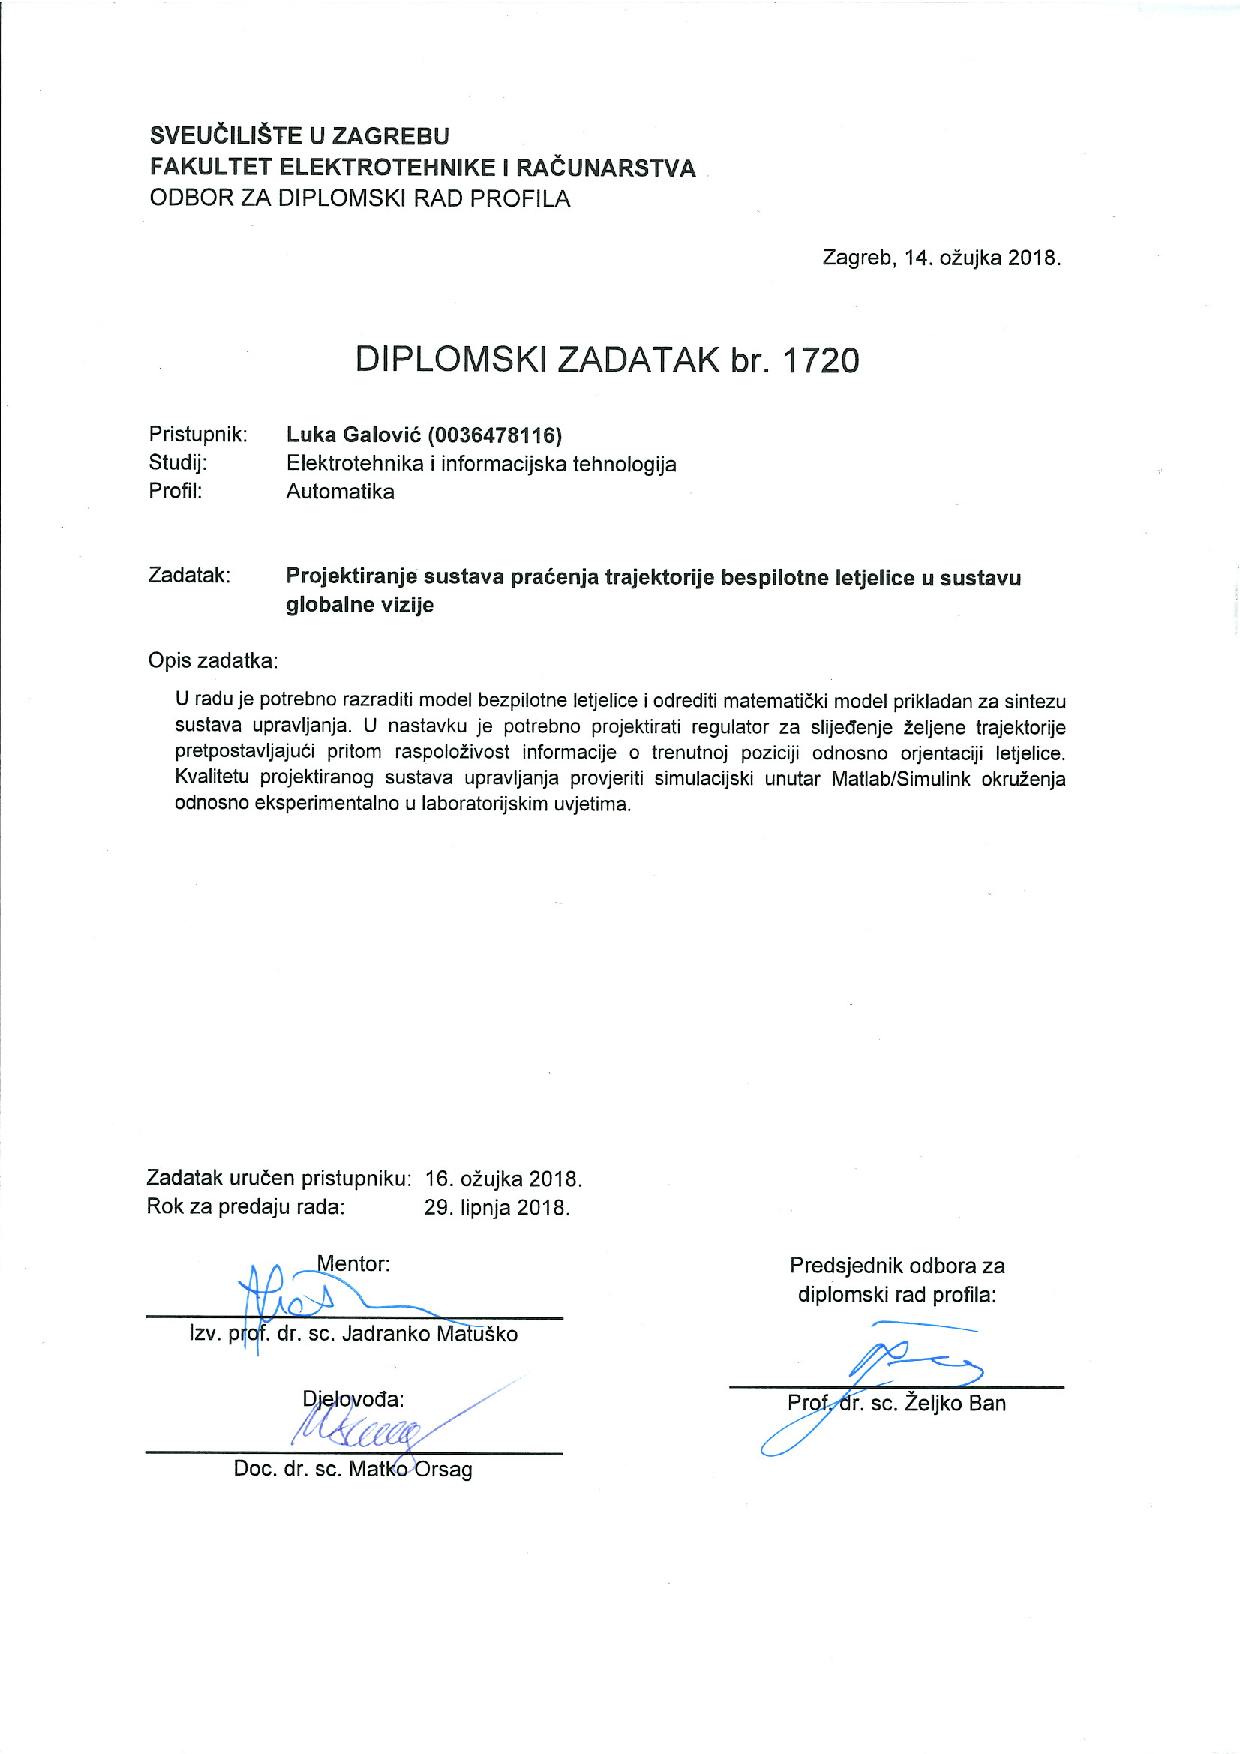
\includepdf[pages=-]{img/izvornik.pdf}

% Dodavanje zahvale ili prazne stranice. Ako ne želite dodati zahvalu, naredbu ostavite radi prazne stranice.
\zahvala{
Veliku  zahvalnost,  u  prvom  redu,  dugujem  svom  mentoru izv. prof. dr. sc. Jadranku Matušku koji mi  je  omogućio  svu  potrebnu  opremu  i  pomogao  svojim  stručnim savjetima  pri  izradi  ovog  diplomskog rada.
	
Također zahvaljujem doc. dr. sc. Šandoru Ilešu na pomoći i stručnim savjetima na nekim ključnim mjestima ovog rada.\\

Zahvalu želim izraziti kolegi Bojanu Spahiji, čiji diplomski rad je vezan za izradu sustava globalne vizije, na strpljenju, podršci te pomoći. \\

Dodatno se  zahvaljujem svim  svojim  prijateljima  i  prijateljicama,  koji  su  uvijek  bili  uz  mene i bez kojih cijeli ovaj tijek mog studiranja ne bi prošao tako lako i zabavno. \\

Posebnu  zahvalnost  iskazujem  cijeloj  svojoj  obitelji  koja  me  je  uvijek  podržavala  i  upućivala na pravi put.

I na kraju, najveću zaslugu za ono što sam postigao pripisujem svojim roditeljima i sestri, koji su 
uvijek bili TU, uz mene, bez obzira da li se radilo o teškim ili sretnim trenucima i bez kojih 
sve ovo što sam dosad postigao ne bi bilo moguće.\\

Velika HVALA svima! }

\tableofcontents
% Tu možete staviti popis slika i tablica
\listoffigures
%\listoftables


\chapter{Uvod}
Ulaskom u novo stoljeće svjedočimo nastavku razvoja, usavršavanja i stvaranja novih tehnologija koja su pomoć u različitim ljudskim aktivnostima. Iako pojam bespilotnih letjelica postoji već dugi niz godina, one su tek u bliskoj prošlosti postale pojam svakodnevnice. Dugi niz godina bespilotne letjelice su se koristile, nažalost, samo u vojnim svrhama zbog čega su stradavali i nedužni civili zbog čega se njihov razvoj držao u tajnosti. Samo saznanje da se koriste u vojsci upućuje na to da je puno vremena i novaca uloženo u njihov razvoj, preciznost, nosivost te izdržljivost.\\
Danas se uz nagli trend upoznavanja s tehnologijama bespilotnih letjelica, kao i digitalnih zapisa i pohranjivanja memorije svakodnevnih događaja namjena korištenja promijenila te su uvedeni novi pojmovi poput \glqq dronovi\grqq --- suvremena riječ koja zapravo opisuje nekoliko vrsta bespilotnih letjelica. Glavna područja njihovih korištenja su: javna sigurnost, zabava, nadzor i inspekcija, informacije, znanost o Zemlji.\\
Korištenje  bespilotnih letjelica, naročito u civilne svrhe, bilježi eksponencijalan rast, kako u pogledu njihovog broja, veličine i težine, tako i u pogledu sve brojnijih mogućnosti njihove primjene \citep{EUR-Lex}. Cilj je razviti jeftinije i sposobnije bespilotne letjelice. U skoroj budućnosti tehnologija će se usavršiti pa će manje letjelice moći prenositi sve veću opremu, tako npr.~poštanski paketi će se dostavljati pomoću letjelica. Motiv izrade ovog rada leži u širokoj primjeni (kako u različitim granama industrije i istraživanja tako i za zabavu). \\
Cilj ovog rada je shvatiti rad bespilotne letjelice te izrada sustava za slijeđenje željene trajektorije. Izazov je kretati se zadanom trajektorijom znajući da postoje razne vanjske smetnje koje utječu na upravljanje. Za to je potrebno implementirati algoritam upravljanja. Cilj upravljanja je stabilizirati sustav oko reference ili prema trajektoriji. To se postiže povratnim informacijama, odnosno mjerenoj poziciji. Za implementaciju algoritma potrebno je dobro razraditi dinamički model. Dronovi imaju šest stupnjeva slobode gibanja i četiri upravljačke veličine, što znači da su dronovi nestabilni sustavi. Jedini pokretni dijelovi su propeleri. U teorijskom dijelu će se opisati razvoj, svrha odnosno tipovi bespilotnih letjelica, dok će se detaljnije razraditi njezin model te odrediti matematički model prikladan za sintezu sustava upravljanja. Projektirat će se regulator za slijeđenje reference, uz pretpostavku raspoloživosti informacije o trenutnoj poziciji te orijentaciji. Provjera projektiranog sustava je provedena eksperimentalno u laboratorijskim uvjetima.

\section{Bespilotne letjelice}
Bespilotne letjelice (UAV\footnote{UAV \engl{Unmanned Aerial Vehicle} – opći je pojam koji označava zapravo sve vrste bespilotnih letjelica koje se kolokvijalno najčešće nazivaju dronovima. Pod tim se obično spominju dvije vrste letjelica kojima ne trebaju ljudski piloti, prve su tzv. kvadrikopteri \engl{quadcopter}, letjelice s četiri elise pomoću kojih dron može lebdjeti na mjestu i kretati se u raznim smjerovima. Drugi tip bespilotnih letjelica su izgleda projektila ili zrakoplova kojim se upravlja iz baze i povezani su uglavnom s vojnim operacijama.}) su, najjednostavnije rečeno, letjelice koje su sposobne izvršiti kontinuirani let bez prisutnosti pilota \citep{UAV}. Postoje razni oblici i veličine, no najčešće su dizajnirane za točno specifične uloge.\\
U nastavku bit će navedeni kratak pregled bespilotnih letjelica kroz povijest, njihova definicija, vrste te primjena.\\
Današnji dronovi su opremljeni raznim senzorima (akcelometri, žiroskop, kamere) koji olakšavaju njihovo upravljanje i točnost pozicioniranja u prostoru.
%Definiranjem pojma bespilotnih letjelica nailazi se na bogat izbor objašnjenja jer imaju široku primjenu. \\

\subsection{Pregled povijesti}
Početak razvoja bespilotnih letjelica je usko vezan s razvojem svih zrakoplova. Povijest seže u prošlo stoljeće kada su Kinezi puštali papirnate zmajeve prema nebu ili letjeli u balonima na vrući zrak, a moglo bi se reći da je prva bespilotna letjelica kamen koji je bacio špiljski čovjek u pretpovijesno doba. Ove \glqq letjelice\grqq imaju malo ili nimalo kontrole. U suvremenom dobu, bespilotnim letjelicama se nazivaju sve letjelice koje su imale autonomno ili daljinsko upravljanje. Razvojem tehnologija i moderniziranjem nazivi i opisi ovih letjelica se mijenjaju --- poput ratnih torpeda, bespilotnih vozila, daljinski upravljača, autonomna kontrola, dron itd.\\
U ranim godinama zrakoplovstva, sama ideja da zrakoplov leti bez ljudskog faktora imala je veliku prednost u tome što je na taj način u potpunosti uklonila rizik za život. No pojavio se veliki nedostatak kod mogućnosti upravljanja takvim letjelicama, odnosno postojala su određena ograničenja. Tako su bespilotne letjelice bile opisane kao 3D \engl{dangarous, dirty, dull} --- opasne, prljave i glupe. Opasne su jer njima netko može srušiti zrakoplov i dovesti u opasnost pilota i ostale putnike, zatim prljave  jer se kreću na mjestima koja su izložena kemijskim, biološkim ili radiološkim opasnostima, te glupe jer je potrebno njima upravljati nekoliko sati što postaje stresno i nepoželjno \citep{unmannedAircraftSystem}. Danas se upotreba i korištenje znatno promijenilo te su one postale popularan izvor zabave, uz svrhu i na nekim drugim područjima.\\
Bespilotne letjelice kao takve, bile su prepoznatljive i prije Prvog svjetskog rata. Tome su  doprinijeli ljudi koji su ih već tad koristili za područje istraživanja i slično. Konkretnije, 1883.  godine  Douglas  Archibald, po  nacionalnosti Englez,  na liniju  „zmaja“  stavio  je anemometar  te  je  mjerio  brzinu  vjetra  na  raznim  nadmorskim  visinama. Nekoliko  godina kasnije, na „zmaj“ je priključio kamere te je na taj način proizveo prvo izviđanje putem letjelice. Nadalje, William Eddy snimio je tisuće fotografija koristeći „zmaj“ s kamerama tijekom rata što se može smatrati prvim korištenjem bespilotnih letjelica za vrijeme ratne borbe \citep{UAVSystems}.\\
Veliki razvoj bespilotnih letjelica vidljiv je u vojne svrhe. Charles  Kettering  razvio  je  bespilotnu  letjelicu  s  dva  krila, tzv.~dvokrilac za tadašnju vojsku (\emph{Army Signal Corps}). Tri godine razvoja dovele su do letjelice nazvane „\emph{Kettering Aerial Torpedo}", odnosno „\emph{Kettering Bug}“ ili samo „\emph{Bug}“. Letjelica je mogla letjeti približno 40 do 55 m/h te nositi oko 80 kg teškog eksploziva. Bila je usmjerena prema cilju sa svojim postavkama i imala  je  odvojiva  krila  koja  bi  se ispustila u  trenutku kada  bi  letjelica  bila iznad  mete dopuštajući trupu aviona da padne na tlo kao bomba.  Također 1917.~, Lawrence Sperry je razvio UAV (vidi \ref{sec:UAV}), sličan kao od Katteringa. Letjelica je imala naziv \emph{Sperry - Curtis Aerial Torpedo}, a bila je namjena za mornaricu. Imala je  nekoliko uspješnih letova, no nikad se nije koristila u ratu. Tvrtka pod nazivom \emph{Radioplane Company} je izradila tisuće ciljnih dronova \engl{target drones} za vrijeme drugog svjetskog rata. Nijemci su u kasnijim godinama drugog svjetskog rata koristili smrtonosne bespilotne letjelice V-1 i V-2. Tek su se u vrijeme Vijetnamskog rata bespilotne letjelice uspješno koristile kao sredstva za nadziranje odnosno izviđanje \citep{UAVSystems}. Značajnu ulogu bespilotne letjelice imale su i u ratovima u Bosni i Afganistanu.\\
Nadalje, tijekom zadnjih nekoliko godina ovakve letjelice su se sve više razvijale i modernizirale te se njihova svrha i način korištenja promijenio. Ovakav razvoj doveo je do pitanja hoće li bespilotne letjelice, odnosno sustavi bespilotnih letjelica, zamijeniti zrakoplove i letjelice za koje je potreban ljudski faktor. Postoje u potpunosti automatizirane letjelice čiji je kontrolni sustav neovisan o vanjskim signalima, a i one koje sadržavaju mogućnosti ručnog upravljanja  od  strane  pilota.  Teoretski,  potpuno  automatizirane  letjelice  mogu  letjeti  bez utjecaja ili ometanja od strane bilo kakvog signala, no njihov nedostatak je taj što mogu biti kontrolirane od strane računala. Na taj način je omogućeno manipuliranje sustavom te unatoč jakoj enkripciji,  još  uvijek  postoji  sigurnosni  rizik  i  opasnost.  Upravo  zbog  toga  te  same kontrole  i  sigurnosti  zrakoplova, i njihovih putnika, odgovornost koju pruža ljudski faktor u zrakoplovstvu, spriječit će da bespilotne letjelice postanu prioritet ili da u potpunosti zamijene normalne letjelice \citep{UAVSystems}.\\
Danas se vojna upotreba bespilotnih letjelica može podijeliti na tri područja, to su pomorska, kopnena i zračna upotreba, dok se u civilne  svrhe  može  upotrijebiti  u  različitim  područjima ljudskih  aktivnosti  kao  npr.  u  geodeziji  tj. fotogrametriji,   poljoprivredi,   industrijskoj proizvodnji,  civilnoj  zaštiti,  upravljanju katastrofama,  zaštiti  okoliša,  nadzorom policijskog    djelovanja,    obavještajnim službama,   novinarstvom,   komercijalnim djelatnostima, razonodom itd. Također  je  sve  veća  uporaba  bespilotnih letjelica za inspekciju   nepristupačnih dijelova  u industrijskim  objektima  kao  što su: brane, dalekovodi, visoki dimnjaci, cjevovodi, mostovi i dr. Isto tako sve su popularniji i mali modeli namijenjeni za razonodu.

\subsection{Definicija bespilotnih letjelica}
Za pojam bespilotnih letjelica koristi se engleski službeni naziv „Unmanned Aerial Vehicle“,  dok  se  zadnjih  nekoliko  godina  pojavio  pojam  UAS  \engl{Unmanned  Aerial System}. Time se htjela naglasiti činjenica da su to složeni sustavi koji uključuju i postaje na zemlji te mnoge druge elemente, a ne samo letjelice koje lete zrakom. Međutim, pojam UAS nije puno korišten za razliku od pojma UAV koji je postao dio modernog leksikona.\\
Bespilotne letjelice lete bez ljudskog pilota, umjesto toga kontrolira ih operator na tlu. Svrha bespilotnih letjelica, odnosno u ovom slučaju se govori o sustavu bespilotnih letjelica (UAS),  tj.  dronova, je  dostava poruke,  paketa  ili  samo  skupljanje  podataka. Kao najvažnija svrha sustava je upravo prikupljanje podataka. Letjelice poput dronova, a i neke druge, mogu prodrijeti  u  područja  i  lokacije  do  kojih  čovjek  ne  može  bez  određene  opasnosti  i  rizika. Ponekad, podaci mogu biti presudni za određene operacije ili aktivnosti. Također, navodi se da je jedna od karakteristika ovakvih sustava to što ih se može ponovno koristiti, odnosno to što se vraćaju (Unmanned Aerial Vehicle Systems Association, 2016).

\subsection{Prednosti i nedostaci}
Postoji nekoliko prednosti i nedostataka koje pružaju bespilotne letjelice. Prednost u odnosu na letjelice s pilotom je upravo u tome, što bespilotne letjelice ne trebaju imati pilota 
koji fizički  mora  biti  unutar  letjelice i upravljati  njome.  Nadalje, jedna od prednosti je ta što mogu doći na nedohvatljiva područja za ljude, a obavljaju precizno i kvalitetno snimanje terena. Mogu ostati u zraku i do 30 sati \citep{AdvantagesofUAS}. Samim time, bespilotna letjelica predstavlja sigurno okruženje te se može kretati dosta velikom brzinom. Ukoliko dođe do pada letjelice, nema štete od stradanja pilota, a uz to mogu letjeti u zonama u kojima postoje velike opasnosti i to na duže vrijeme \citep{Soffar}.
Prednosti koje dronovi pružaju su njihova niska cijena te je održavanje puno jeftinije od običnih letjelica i zrakoplova. Uz to, dronovi mogu letjeti na niskim nadmorskim visinama za razliku od zrakoplova, a također mogu letjeti nekoliko sati bez prestanka. Njihove sposobnosti snimanja, nadziranja, nadgledavanja, izviđanja jedne su od velikih prednosti kao i laka i brza implementacija sustava \citep{PhilForHumanity}.\\
S  druge  strane,  postoje  i  neki  nedostaci  bespilotnih  letjelica  i  dronova. Bespilotne letjelice su u odnosu na dronove, skupe za proizvodnju, dok se veliki troškovi mogu pojaviti i ljudskom greškom kod letjelica s daljinskim upravljanjem te to može uzrokovati njen pad. Također, može se dogoditi i to da se letjelica izgubi što također donosi velike troškove. Kvarovi na računalu isto mogu uzrokovati štete na bespilotnim letjelicama, naročito kada se one koriste za vojne napade što može rezultirati ubijanjem civila i uništenjem  civilne  imovine \citep{Soffar}. \\
Unatoč tome, vojska i dalje koristi dronove i  bespilotne letjelice jer vjeruju u njihove prednosti, a nisu svjesni nedostataka. Nedostaci dronova su ti da oni ne mogu komunicirati s civilima, odnosno u slučaju vojnog napada te potrebe za evakuacijom nekog područja. Loše programirani dronovi mogu izazvati velike štete, a kao takvi mogu biti preuzeti od strane neprijatelja što dovodi u pitanje sigurnost takvih sustava. 


 

\subsection{Vrste}
Prema \citet{UAVSystems} postoje  3  vrste  letjelica  bez  pilota,  isključujući 
projektile: \begin{itemize}
\item Bespilotne letjelice \engl{Unmanned Aerial Vehicle - UAV} (slika \ref{fig:UAV letjelica})
\item Letjelice na daljinsko upravljanje \engl{ Remotely Piloted Vehicle - RPV} (slika \ref{fig:RPV letjelica})
\item Dronovi \engl{Drones} (slika \ref{fig:dron})
\item Oblik kukca \engl{insect fly shaped drone} (slika \ref{fig:oblik kukca})
\end{itemize}
\begin{figure}[htb]
\centering
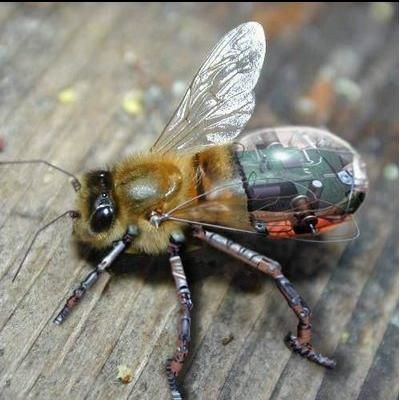
\includegraphics[width=6cm]{img/insect_fly_shaped_drone.png}
\caption{Letjelica oblika kukca\protect\footnotemark}
\label{fig:oblik kukca}
\end{figure}
\footnotetext{Izvor: https://i.pinimg.com/474x/dd/6c/65/dd6c65f6342309d5fe1027ad3cd66a20--spy-gadgets-radio-control.jpg}
U današnje doba, najčešći pojam koji se javlja za opisivanje bespilotnih letjelica je dron. Razlika između drona i bespilotne letjelice (UAV) je u stupnju automatizacije, jer dronov let ovisi o unaprijed programiranom ponašanju, a kod UAV postoji daljinsko upravljanje od strane pilota  u  kontrolnoj  stanici \citep{UAVInsider}. U ovom radu bit će naglasak na treću vrstu bespilotnih letjelica koje se sve više i više danas koriste, a to su dronovi. 

\subsubsection{UAV}\label{sec:UAV}
Kao što je već spomenuto, bespilotna letjelica je letjelica ili zrakoplov bez pilota. Njome se može upravljati na daljinski, odnosno od strane osoba koja to čini u kontrolnoj stanici. S druge strane, može letjeti samostalno na temelju unaprijed programiranih planova leta ili više složenih dinamičkih sustava za automatizaciju. Takve letjelice se koriste za mnoge svrhe i misije, najčešće u slučaju izviđanja, no ponekad imaju i napadačke uloge. Sposobnosti koje posjeduje su te što može biti kontrolirala, ima održiv horizontalni let i pokreće se pomoću mlaznog ili klipnog motora. Postoji nekoliko tipova ovakvih letjelica, a klasificirane su prema svrsi koju obavljaju:
\begin{itemize}
\item Za pronalaženje ciljeva i meta --- pronalazi zemaljske i zračne neprijateljske mete 
\item Izviđačke --- omogućuje pronalazak ratnih polja
\item Za borbu --- ima napadačku sposobnost za visoko rizične misije
\item Za istraživanje i razvoj --- koristi se za daljnji razvoj tehnologije
\item U građanske i trgovačke svrhe --- posebno dizajniran za državne i komercijalne svrhe
\end{itemize}
Neke  od  bespilotnih  letjelica  su:  Altair,  Global  Hawk,  X47-A, Prowler II, X45-A UCAV, Fire Scout, Predator A i Predator B, ER/MP UAS, I-GNAT, Mariner, Army I-GNAT ER i drugi.
\begin{figure}[htb]
\centering
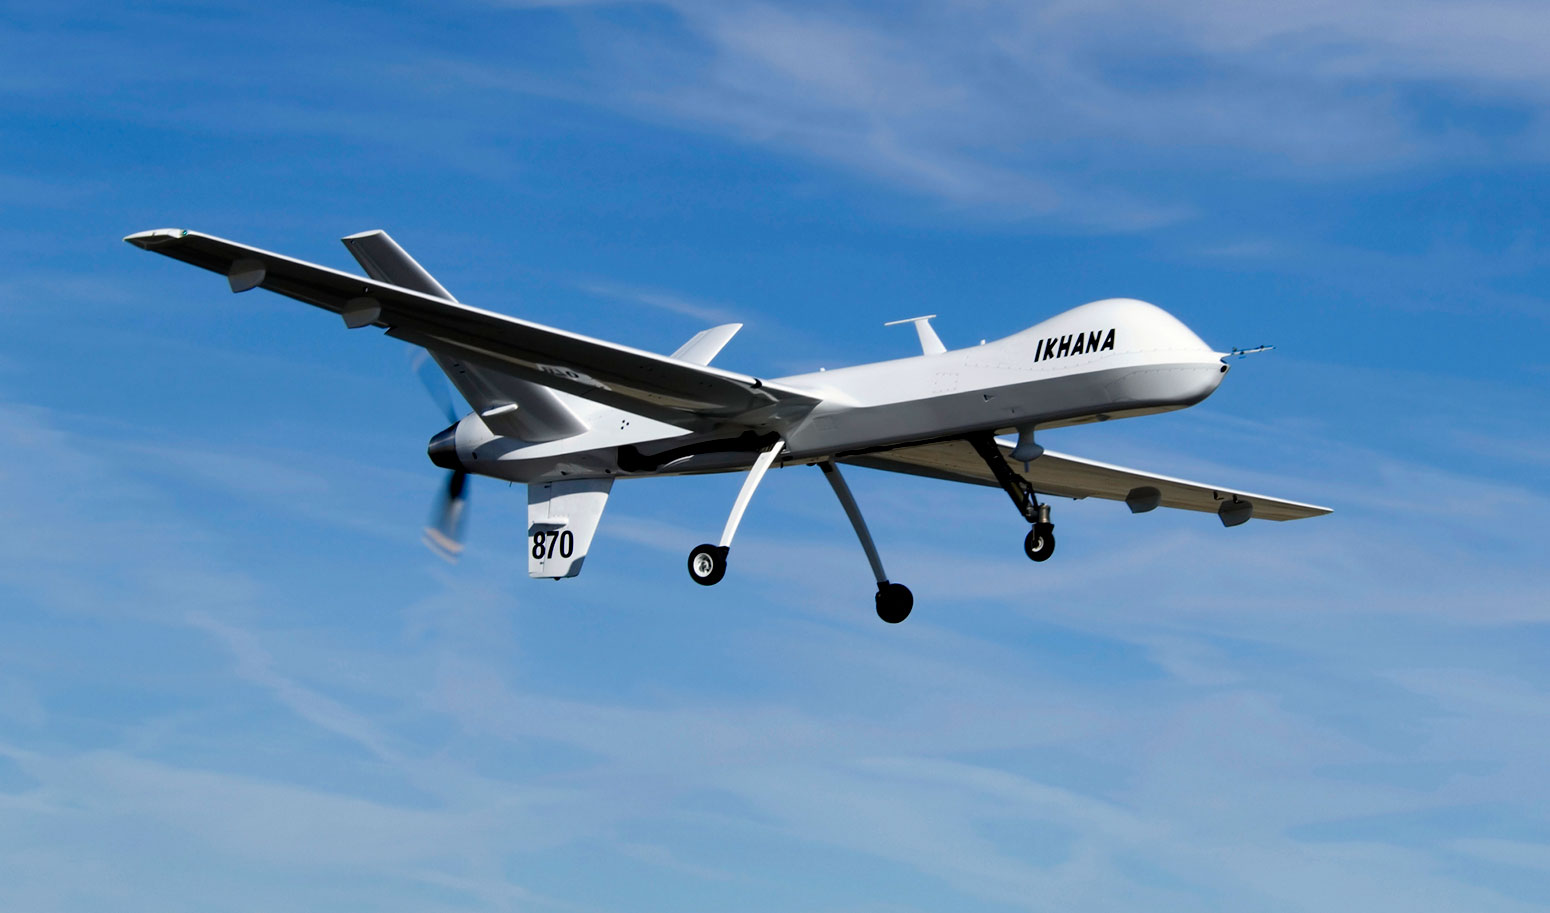
\includegraphics[width=8cm]{img/UAV.png}
\caption{UAV letjelica\protect\footnotemark}
\label{fig:UAV letjelica}
\end{figure}
\footnotetext{Izvor: https://www.mitre.org/sites/default/files/images/uas-track-civil-airspace-aviation.jpg}

\subsubsection{RPV}
RPV su letjelice na daljinsko upravljanje \engl{ Remotely Piloted Vehicle}. Takve male letjelice  su  najviše  korištene  za  terenski  rad  vezan  uz  okoliš. Prema  tome,  njihov  raspon korištenja kreće se od šumarstva, morskih istraživanja, promatranja biljnih i životinjskih svijeta, dobivanja uzoraka o biološkim stvarima iz zraka i slično. Prednosti takvih letjelica su u tome što je pilot siguran, odnosno nije fizički prisutan. Zatim, brzo prikupljanje podataka, niska cijena te relativno kratko vrijeme odaziva i dobivanja odgovora na zahtjeve. No s druge strane, postoje i neka ograničenja prilikom takvih letjelica, a to su niska stabilnost kao fotografske platforme, kratko vrijeme leta, malobrojnost senzora, teškoće kod navigacijskog sustava itd. \\
Daljnji razvoj i korištenje letjelica na daljinsko upravljanje je upravo za potrebe snimanja stanja okoliša. Osim otkrivanja i procjene okoliša, potreban je i daljnji fokus na poboljšanje slike te omogućiti ugradnju više senzora za razna mjerenja \citep{Hardin}.
\begin{figure}[htb]
\centering
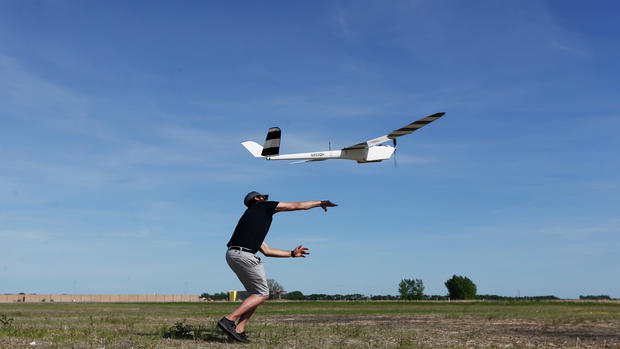
\includegraphics[width=8cm]{img/RPV.png}
\caption{RPV letjelica\protect\footnotemark}
\label{fig:RPV letjelica}
\end{figure}
\footnotetext{Izvor: http://www.grandforksherald.com/sites/default/files/styles/16x9\_620/public/field/image/060916.n.gfh-\_.grandsky\%20001.JPG?itok=iMeyXr2z}

\subsubsection{Dronovi}
Vrsta bespilotnih letjelica, poznatijih kao dronovi su zračni bespilotni sustavi koji mogu biti kratkog ili dugog dometa, a koriste se za vojne ili civilne svrhe. Najčešća oprema koju dron sadržava je kamera, a neki mogu biti naoružani projektilima. 
\begin{figure}[htb]
\centering
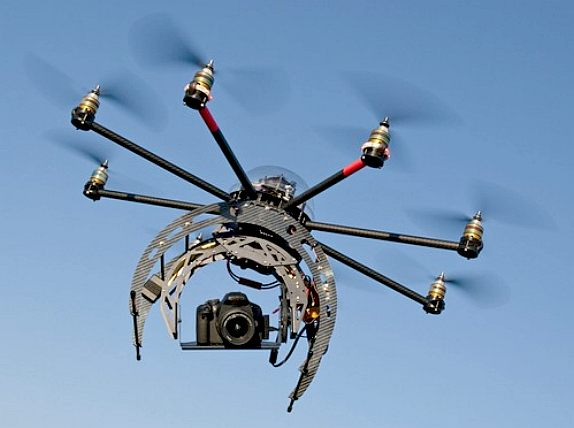
\includegraphics[width=8cm]{img/drone.png}
\caption{Dron\protect\footnotemark}
\label{fig:dron}
\end{figure}
\footnotetext{Izvor: http://www.bluebird-electric.net/artificial\_intelligence\_autonomous\_robotics/robotics\_artificial\_intell-igence\_autonomous\_pictures/uav\_drone\_photo\_recon\_camera\_multi\_rotor\_helicopter.jpg}
Na  slici~\ref{fig:dron}  nalazi  se  slika 
drona. Današnja najvažnija primjena dronova je stvaranje mapa, odnosno snimaka iz zraka. Dronovi su  vrlo dobri u izradi karata, daleko više od drugih tehnologija za istu primjenu. Nadalje, odlični su u fotografiranju i računalnoj  obradi  tih  fotografija \citep[str.~10]{Drones}. Većina dronova koriste razne senzore kako  bi  napravili  procjenu  stanja,  odnosno  koriste  MEMS \engl{Microelectromechanical} čipove  za  mjerenje  ubrzanja  i rotacije. Neki od njih nose sustav za mjerenje udaljenosti od tla te također mogu imati barometre za  mjerenje  tlaka  zraka.  Uz  to,  dronovi  mogu  imati  na  sebi senzore  za  prijenos  topline  pa  i manetometre za mjerenje zemljinog magnetskog polja. No najveća većina njih posjeduje GPS senzore jer MEMS senzori koji se koriste na takvim jeftinim letjelicama nisu dovoljni precizni. No, GPS ne može ažurirati svoju poziciju dovoljno često te ima svoje oscilacije pa je najbolja kombinacija  upravo  spomenutih  senzora \citep[str.~13]{Drones}.\\
Nadalje, na slici~\ref{fig:konfiguracijaDrona} nalazi se primjer jedne od konfiguracija drona s više motora. Sastoji  se  od  spomenutih  motora  i  propelera,  kontrolera  za  let,  GPS  senzora,  baterije, elektroničkog kontrolera za brzinu, prijemnika, ploče za napajanje i telemetrijskog modula. 
\begin{figure}[htb]
\centering
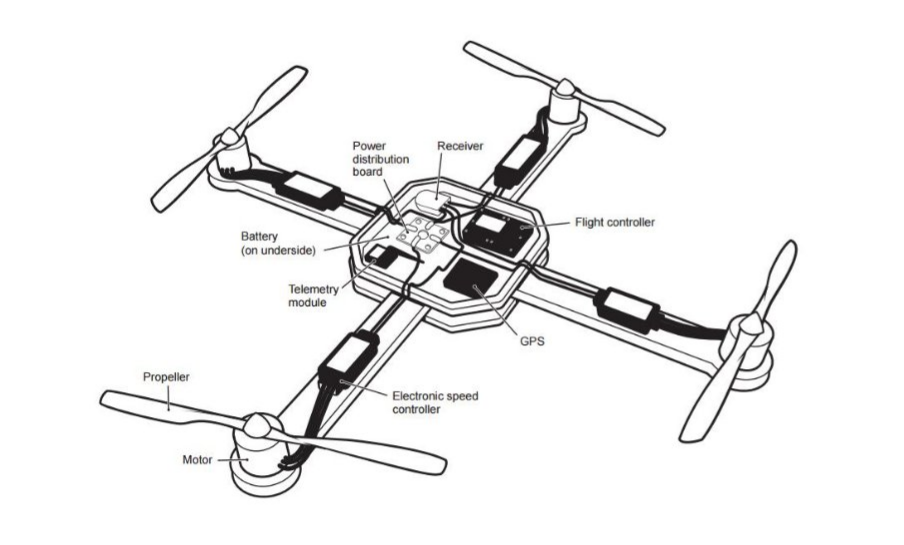
\includegraphics[width=13cm]{img/konfiguracijaDrona.png}
\caption{Konfiguracija drona\protect\footnotemark}
\label{fig:konfiguracijaDrona}
\end{figure}
\footnotetext{http://drones.newamerica.org/primer/DronesAndAerialObservation.pdf}

\subsection{Zakonska regulativa \citep{Ekscentar}} 
Bilježenjem nezakonitih upotreba bespilotnih letjelica u kojima su ugroženi ljudski životi i koji nisu u skladu s određenim zakonima (zakon o zaštiti osobnih podataka), kako bi se ograničila i osigurala upotreba bespilotnih letjelica potrebna je zakonska regulativa o toj temi. S obzirom na to da korištenje dronova, povećanjem njihovog broja, prvenstveno za zabavu postaje veoma popularno i u Republici Hrvatskoj, javlja se potreba za razmatranje zakonske regulative\footnote{Zakon o dronovima: \url{http://www.dronovi.hr/zakon-o-dronovima.html}}.  Letjelice  se  mogu  vrlo  lako  nabaviti  ili  izraditi  te  postoji mogućnost preplavljenosti zračnog prostora. Zbog toga je potrebno registrirati svaku letjelicu i regulirati njezinu uporabu. Tako je prema Pravilniku o sustavima bespilotnih zrakoplova utvrđeno, osim općih odrednica o klasama područja letenja i letačkih operacija te veličine samih bespilotnih letjelica, to da se let bespilotnim letjelicama smije odvijati samo danju. Nadalje, potrebno je osigurati sigurnu udaljenost letjelice od ljudi, objekata, vozila, cesta, dalekovoda i drugo. Rukovoditelj bespilotne letjelice mora od nje biti udaljen do 500 metara te mu ona uvijek mora biti unutar vidnog polja. Što se tiče zrakoplova, let  drona  mora  biti  udaljen  najmanje  3  kilometara  od  aerodroma.  Dakako,  zabranjeno  je izbacivanje bilo kakvih predmeta iz letjelice. \\
No kako se dronovi najčešće koriste za snimanja iz zraka, postoje zakoni koji se moraju poštovati i za to. Dakle, navodi se da snimati iz zraka smiju pravne i fizičke osobe koje su za to pravodobno registrirane. Zatim je potrebno podnijeti zahtjev za izdavanje odobrenja za snimanje s dostavom  raznih  podataka (geodetsko snimanje koje se predaje Državnoj geodetskoj upravi):
\begin{itemize}
\item podatke o naručitelju snimanja
\item podatke o izvršitelju snimanja i dokaz o registriranoj djelatnosti iz zraka izvršitelja snimanja (potrebno priložiti kopiju registracije pri Trgovačkom sudu)
\item podatke o izvršitelju razvijanja
\item podatke o vremenu snimanja
\item svrhu snimanja
\item popis objekata, skicu ili kartu s označenim područjem snimanja
\item podatke o vrsti i mjerilu snimanja, kameri, žarišnoj daljini objektiva, filmu ili obliku zapisa (analogni/digitalni)
\item način čuvanja izvornih podataka snimanja.
\end{itemize}
Tek nakon dobivanja odobrenja može se pristupiti snimanju te kasnije i razvijanju zračnih snimaka i pri tome je dužna najkasnije u roku od 8 dana od dana snimanja dostaviti zračne snimke na pregled Državnoj geodetskoj upravi (Zakon o obrani, NN 33/02), dok je za bilo kakvo umnožavanje, objavljivanje ili iznošenje snimaka iz Hrvatske potrebno  pribaviti  odobrenje  uz  suglasnost  ministarstva (Ministarstvo  pomorstva,  prometa  i infrastrukture, 2015).\\
Prilikom snimanja iz zraka pojedinih vojnih, telekomunikacijskih, energetskih i industrijskih objekata, područja nacionalnih parkova i parkova prirode te drugih zaštićenih dijelova prirode, također je potrebno priložiti i mišljenje korisnika objekta, odnosno ustanove koja upravlja zaštićenim dijelom prirode (Uredba o snimanju iz zraka, NN 116/03). Digitalni oblik obrasca Zahtjeva za izdavanje odobrenja za razvijanje zračnih snimaka može se pronaći na službenim internetskim stranicama Državne geodetske uprave, a uz obrazac je potrebno priložiti dokaz o registriranoj djelatnosti za snimanje iz zraka, dok je za letjelicu potrebno priložiti kopiju Certifikata za obavljanje radova iz zraka s Operativnim specifikacijama koju izdaje Agencija za civilno zrakoplovstvo.\\

\subsection{Primjena i rasprostranjenost}
Kako bespilotne  letjelice  postaju  manje,  jeftinije  i  jednostavnije za  upravljanje,  a regulativne izmjene, naročito u SAD-u, smanjuju prepreke za nove korisnike, letjelica je sve više. 
Prema izvješću tvrtke PwC (Price Waterhouse Coopers) “Clarity from above“ može se govoriti o globalnoj tržišnoj vrijednosti rješenja baziranim na bespilotnim letjelicama višoj od 127,3 milijardi dolara.
Očekuje se da će se povećanjem broja letjelica smanjiti nesreće na radu, 
poput pada zaposlenika s krova tijekom inspekcija zgrada, a time i gubici zbog kompenzacija 
radnicima. 
Bespilotne letjelice bi u budućnosti mogle riješiti niz problema i smanjiti troškove i u nizu drugih industrija, u zemljama u razvoju i slučajevima prirodnih katastrofa. \citep{Allianz}
Kao što je navedeno ranije, postoji podjela bespilotnih letjelica (UAV) prema njihovoj svrsi. Tako  su  najprije  bile  namijenjene za korištenje u vojne svrhe, no danas je njihova primjena puno veća \citep{TheUseOfUAS}. Ostala područja u kojima se danas koriste su:\begin{itemize}
\item geodezija --- projektiranje, rudarstvo, geologija, šumarstvo
\item poljoprivreda
\item kotrola i nadzor nad kritičnom infrastrukturom
\item sigurnost i okoliš
\item praćenje i nadzor okoliša
\item potraga i spašavanje
\item sigurnost
\item dostava
\end{itemize}
U  vojne  svrhe bespilotne  letjelice  se  koriste  za  sigurnosni  nadzor  i  kontrolu  vojnih područja, za zračne izvidnice, otkrivanje kemijskih, bioloških, radioloških i nuklearnih uvjeta na nekom terenu, zatim za telekomunikacijski promet, za potragu i spašavanje i dr. Što se tiče terenskog  pretraživanja  i  spašavanja,  vrše  nadgledanje  i  obilježavaju  točke  na  kojima  je potrebna intervencija i slično. Nadalje, bespilotne letjelice  su  korisne  i  u  telekomunikacijske svrhe, a čak mogu i detektirati lansiranje nekog projektila \citep{Military}.\\
U poljoprivredi se pomoću dronova ili drugih vrsta bespilotnih letjelica za tu svrhu, nastoji povećati produktivnost i efikasnost  proizvodnje.  Dronovi  se  mogu  koristiti  za  nadzor usjeva,  provjeru  uvjeta  na  zemljištu  da  bi  se  tako  ostvario  ekološki  održiv  način  rada,  tj. racionalnije koristila voda, upotrebljavali pesticidi pa i pametnije koristili strojevi.
\begin{figure}[htb]
\centering
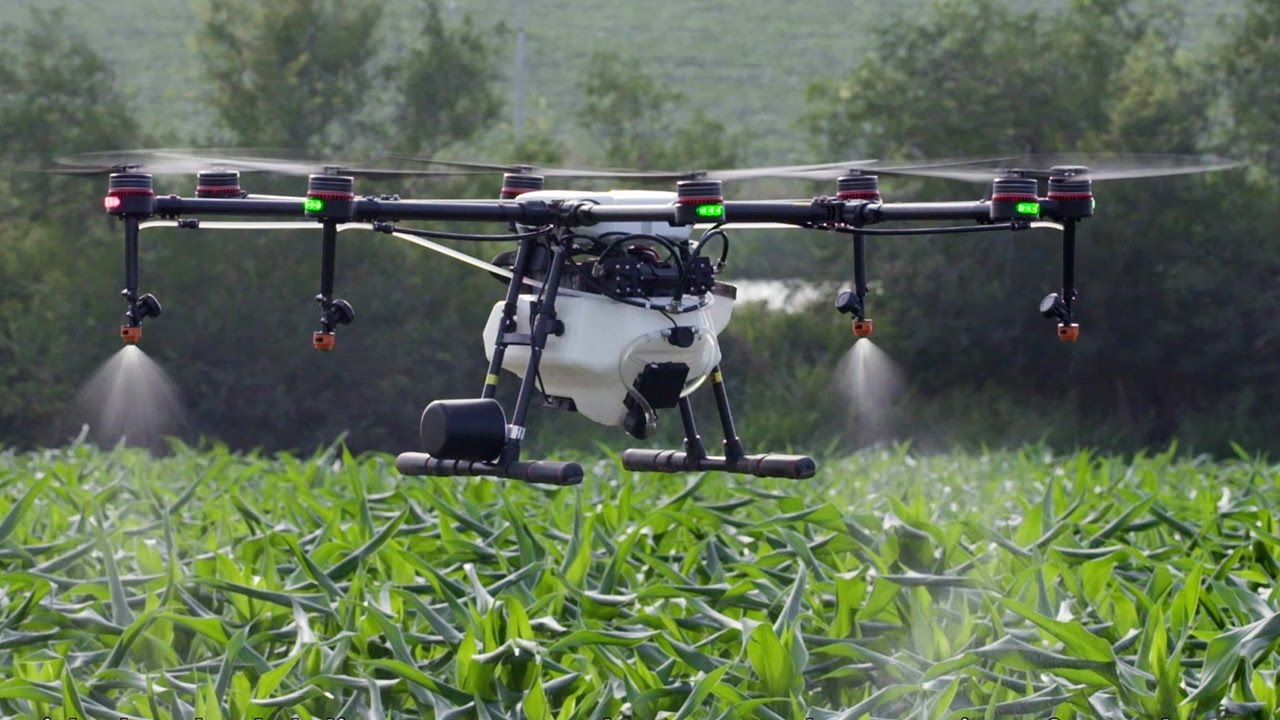
\includegraphics[width=8cm]{img/poljoprivreda.png}
\caption{Upotreba letjelica u poljoprivredi\protect\footnotemark}
\label{fig:letjelicaUPoljoprivredi}
\end{figure}
\footnotetext{Izvor: https://geospatialmedia.s3.amazonaws.com/wp-content/uploads/2017/08/140911-drones-editorial.jpg}
U geodeziji, bespilotne letjelice mogu snimati teren te se na temelju toga može izraditi 3D prikaz, razni digitalni modeli terena i površine itd. Dronovi su korisni jer mogu doći do nepristupačnih terena i područja te obaviti potrebno snimanje  i mjerenje.  Nadalje,  bespilotne letjelice  mogu  biti korisne kod mjerenja infrastrukture i vrše točan, brz i pouzdan nadzor nad objektima zajedno sa preciznim i učinkovitim ugrađenim kamerama \citep{GeoTron}.\\
Praćenje  okoliša,  snimanje  šuma,  procjena  kvalitete  zraka,  kontrola   i nadzor nad kritičnom infrastrukturom (npr.~odlagališta  i otpadne  vode)  te  mnoge  druge  mogućnosti  vezane  uz  okoliš  karakteristične  su za  dronove. Prednost je u tome što takva snimanja i prikupljanja podataka nisu skupa te ne postoje veliki financijski troškovi, a ne ovise niti o vremenskim uvjetima.\\
Također, bespilotne letjelice se koriste i za civilnu sigurnost jer se mogu koristiti za policijski nadzor, zaštitu državnih granica te razne druge nadzore i operacije \citep{GeoTron}. Uz sve navedeno, većina današnjih korisnika, kupuje i koristi dronove ponajviše za zabavu sa željom prikupljanja fotografija s određenih visina. 
Najnovije upotrebe uključuju dostavljanje krvi i cjepiva na udaljene lokacije u Africi, gašenje požara, kontrolu štetnika, pa čak i dostavljanje u ugostiteljskim zanimanjima kao što je dostava hrane.
Osiguratelji  sve  češće  upotrebljavaju ovaj  tip  letjelica za  jednostavniju  i  sigurniju procjenu rizika građevinskih ili infrastrukturnih projekata.

\subsection{Proizvođači}
Danas  najvećim  proizvođačem  bespilotnih  letjelica  za  civilnu  upotrebu  smatra  se kineska kompanija DJI, sa sjedištem u gradu Shenzhen-u. Drugi poznatiji proizvođači su još francuski  Parrot,  odnosno njezina  švicarska  podružnica  senseFly,  američki  3D  Robotics,  kanadski  Aeryon itd.
Bespilotne letjelice  s  kamerama  i  senzorima pružaju poduzećima  diljem  svijeta potpunije podatke.Također se koriste u prijevozu i preciznim poslovnim aktivnostima te tako sve više utječu na poslovne strategije poduzeća.\\
Na  drugoj  po  redu  „The  Commercial  UAV  Show"  konferenciji  u  Londonu održanoj 2015. godine izlagalo je  stotinjak tvrtki iz cijelog svijeta. Korisnici su prezentirali projekte s bespilotnim  letjelicama  uz  mnoštvo  savjeta  kako  započeti  projekte,  kako  ih  prezentirati, implementirati te dijelili konkretna iskustva iz provedenih projekata. Dominirala su rješenja za preciznu  poljoprivredu,  snimanje  arheološke  baštine,  geodetske  izmjere,  izrada  karata  i modeliranje, nadzor okoliša, požarišta, prometnica te razne inspekcije, a pojavio se i značajan broj  specijaliziranih  tvrtki  za  senzore,  motore,  antene  i  ostale  dijelove  bespilotnih  letjelica.(Tihomir Šašić, 2015.)

\subsection{Klasifikacija}
Postoji  veliki  broj  različitih  tipova  bespilotnih  letjelica  s  različitim  mogućnostima, ovisno o potrebama samih korisnika, no ne postoji njihova opće prihvaćena podjela.\\
Europska  zajednica  za  bespilotne  letjelice  \engl{European  Association  of  Unmanned Vehicles Systems - EUROUVS} kreirala je klasifikaciju bespilotnih letjelica na osnovu sljedećih parametara:  visina  leta,  trajanje  leta,  brzina,  maksimalna  nosivost  \engl{Maximum  takeoff weight – MTOW}, veličina letjelice, domet signala i dr. \\
Po  namjeni  bespilotne  letjelice
možemo  podijeliti  na  vojne  i  civilne,  a  civilne  na komercijalne i nekomercijalne. Po namjeni se ove letjelice mogu podijeliti i u četiri glavne kategorije:\begin{itemize}
\item mikro/mini (MAV/Mini) --- najmanje platforme koje lete na najmanjim visinama,
\item taktičke (TUAV),
\item strateške,
\item bespilotne letjelice s posebnom zadaćom
\end{itemize}

\begin{table}[htbt]
\caption{Klasifikacija bespilotnih letjelica prema EUROUVS}
\label{tbl:klasifikacija}
\centering
\begin{tabular}{|M{2.5cm}|M{3cm}|M{2cm}|M{2cm}|M{2cm}|M{2cm}|}\hline
  & Kategorija & Max. nosivost (kg) & Visina leta (m) & Trajanje leta (m) & Domet signala (km)\\ \hline
\multirow{2}{*}{Mini/mikro} & mikro & $0.10$ & $250$ & $1$ & $<10$ \\ \cline{2-6}
& mini & $<30$ & $150-300$ & $<2$ & $<10$ \\ \hline
\multirow{6}{*}{Taktičke} & Bliskog doleta & $150$ & $3000$ & $2-4$ & $10-30$ \\ \cline{2-6}
& Kratkog doleta & $200$ & $3000$ & $3-6$ & $30-70$ \\ \cline{2-6}
& Srednjeg doleta & $150-500$ & $3000-5000$ & $3-10$ & $70-200$ \\ \cline{2-6}
& Dugog doleta & $-$ & $5000$ & $6-10$ & $200-500$ \\ \cline{2-6}
& Dugog doleta i trajanja leta & $500-1500$ & $5000-8000$ & $12-24$ & $>500$ \\ \cline{2-6}
& Srednje leteće dugog trajanja leta & $1000-1500$ & $5000-8000$ & $12-24$ & $>500$ \\ \hline
Strateške & Visoko leteće dugog trajanja leta & $2500-12500$ & $15000-20000$ & $12-48$ & $>500$ \\ \hline
\multirow{4}{2cm}{Bespilotne letjelice s posebnom zadaćom} & Smrtonosne & $250$ & $3000-4000$ & $3-4$ & $300$ \\ \cline{2-6}
& Mamci & $250$ & $50-50000$ & $<4$ & $0-500$\\ \cline{2-6}
& Stratosferske & U razvoj & $20000-30000$ & $>48$ & $>2000$\\ \cline{2-6}
& Egzosferske & U razvoju & $>30000$ & U razvoju & U razvoju \\ \hline
\end{tabular}
\end{table}
Po načinu kontrole i upravljanja bespilotne letjelice dijelimo  na  autonomne  sustave, sustave   samoupravljanja,   sustave   upravljanja   po   radarskom   ili   radio   snopu   (sustav telenavođenja),   sustave   telekomandnog   upravljanja   i   kombinirane   sustave   (autonomni, neautonomni). \citep{Vindis}\\
Prema visini leta, težinu pri polijetanju i maksimalnom doletu bespilotne letjelice možemo podijeliti na (BHDCA, 2016): \begin{itemize}
\item Kategorija  1  (masa  do  1  kg,  visina  leta do 50 m iznad površine \engl{AGL - Above Ground Level}, dolet do 150 m),
\item Kategorija 2 (masa veća od 1 kg do 5 kg, visina leta do 150 m AGL, dolet do 500 m),
\item Kategorija 3 (masa veća od 5 kg do 20 kg, visina leta do 300 m AGL, dolet do 2500 m),
\item Kategorija 4 (masa veća od 20 kg, visina leta veća od 300 m AGL, dolet veći od 2500 m).
\end{itemize}
Po konstruktivnoj izvedbi bespilotne letjelice možemo podijeliti na letjelice koje ostvaruju uzgon potreban za let na:\begin{itemize}
\item Fiksnim aeroprofilnim površinama tj. krilima (zrakoplovi),
\item Rotirajućim  aeroprofilnim  površinama  tj.  elisama  (helikopteri,  heksakopteri ,multirotori) 
\end{itemize}
Prema  međunarodnoj  organizaciji  za civilno  zrakoplovstvo  \engl{International  Civil Aviation Organization - ICAO} bespilotne letjelice mogu se podijeliti u dvije kategorije:\begin{enumerate}
\item Autonomne letjelice --- temelje se na naprednim sustavima za dinamičko navođenje te se trenutačno smatra neprikladnim za regulaciju u civilnom zrakoplovstvu radi zakonskih problema te pitanja odgovornosti.
\item Letjelice na daljinsko upravljanje (RPA) --- letjelice na daljinsko upravljanje podliježu pravnim  potpisima  kao  Međunarodne organizacije  za  civilno  zrakoplovstvo  tako  i propisima  i  zakonima  nacionalnih  agencija  za  civilno  zrakoplovstvo.  Letjelice  na daljinsko upravljanje mogu se podijeliti na one sa fiksnim krilima, rotacijske te ostale modele.
\end{enumerate}
Danas  se  u  civilne  svrhe  najčešće  primjenjuju  mini  i  mikro bespilotne  letjelice  s propelerima  tzv.  ~dronovi.  Razvojem  tehnologija  i  pojeftinjenjem  sustava  za  izvođenje letova  bez  pilota  u  zrakoplovu  takvi  sustavi  su  danas  ekonomski  prihvatljivi  za  razne namjene. 


\section{Sustav za regulaciju}
\subsection{Osnovni pojmovi}
\begin{description}
\item[Automatska regulacija:] po definiciji je automatsko održavanje željenog stanja nekog procesa ili  mijenjanje  tog  stanja  po  određenom zakonu,  bez obzira  na  djelovanje  vanjskih  i unutarnjih  poremećaja.  To  se  postiže  pomoću povratne  veze,  koja  omogućava  usporedbu izmjerene  vrijednosti  neke  veličine  reguliranog  procesa  sa  njenom  željenom  vrijednosti (referencijom),  te  se  na  temelju  razlike  tih  dviju veličina  odlučuje  kako  proces  usmjeriti. Proces  se  usmjerava  upravljanjem  tokom  energije  ili tvari. Regulacija se odvija u „zatvorenom krugu“.
\item[Signal:] funkcija koja opisuje vremensku promjenu fizičke veličine nekog fizičkog procesa. 
\item[Sustav \engl{system}:] skup elemenata povezanih vezama kojima djeluju jedan na drugi.  Sustav  obično 
opisuje fizički proces, uređaj ili međusobnu vezu uređaja.
\item[Ulaz ili pobuda:] Signal  koji  se  može  prepoznati  kao  uzrok  nekih  promjena  u  sustavu.
\item[Izlaz ili odziv:] Signal koji se prepoznaje kao posljedica.
\item[Proces:] općenito  skup  aktivnosti  kojima  se  ulazni  elementi  transformiraju  u  izlazne elemente  sa  specifičnim  svojstvima,  a  sama    transformacija  određena  je  parametrima  i ograničenjima.
\end{description}  

\subsection{Sinteza regulatora}
Sustav upravljanja na temelju (mjerenih) signala ulaza i izlaza procesa pronalazi upravljačke signale koji ostvaruju željeni cilj upravljanja. Linearni sustavi su oni sustavi čije se vladanje može opisati linearnim diferencijalnim jednadžbama (vremenski kontinuirani linearni sustavi) ili linearnim jednadžbama diferencija (vremenski diskretni linearni sustavi).\\
Osnovna struktura sustava upravljanja ilustrirana je na slici \ref{fig:Osnovna struktura} Regulacijski krug sadrži 4 glavna sastavna dijela: proces, mjerni član, regulator, i izvršni (postavni) član.
\begin{figure}[htb]
\centering
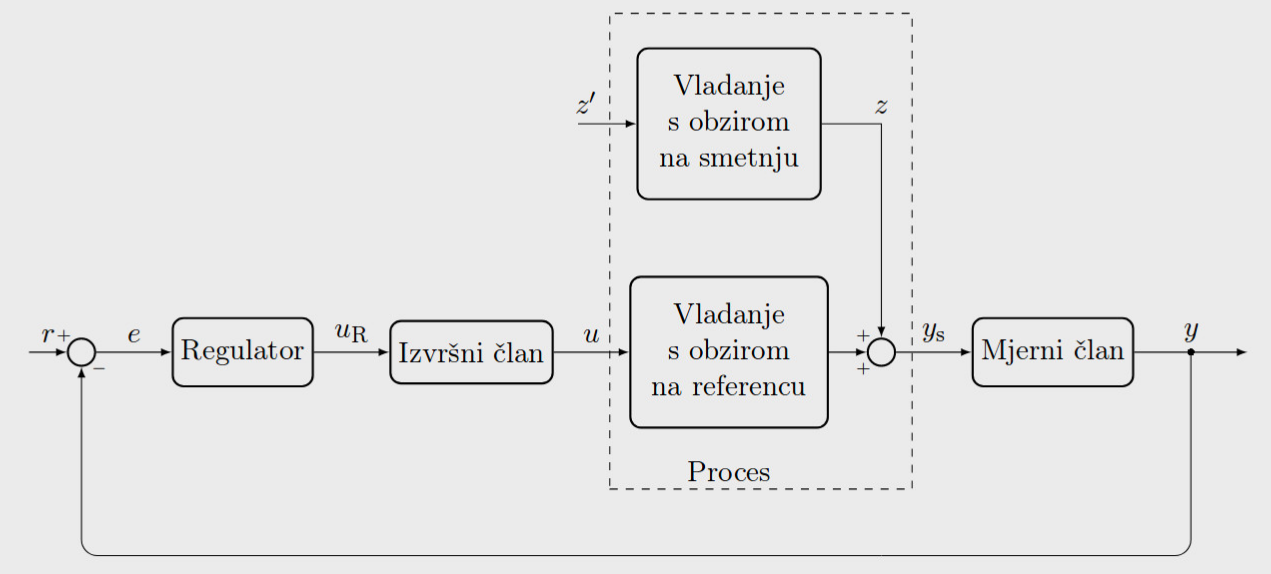
\includegraphics[width=10cm]{img/osnovnaReg.png}
\caption{Osnovna struktura sustava upravljanja\protect\footnotemark}
\label{fig:Osnovna struktura}
\end{figure}
\footnotetext{Izvor: http://www.fer.unizg.hr/\_download/repository/SLSU\_SveucilisniPrirucnik\_2018\_05\_18.pdf}\\
Sa stajališta projektiranja sustava upravljanja praktičnije je razmatrati pojednostavljenu shemu sustava upravljanja (vidi sliku \ref{fig:Pojednostavljena struktura}) kod koje su regulator i izvršni član objedinjeni, a mjerni član je idealan.
\begin{figure}[htb]
\centering
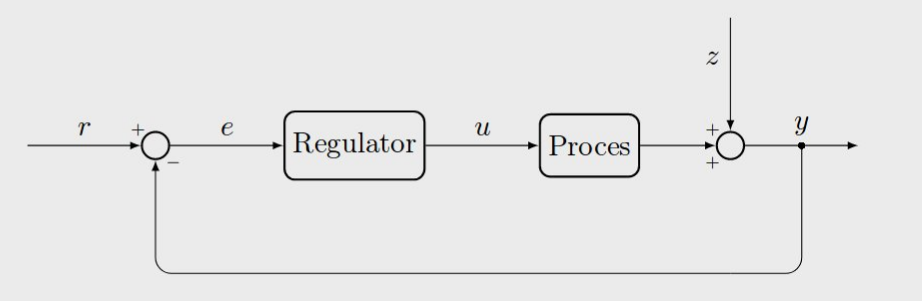
\includegraphics[width=10cm]{img/struktura.png}
\caption{Pojednostavljena struktura sustava upravljanja\protect\footnotemark}
\label{fig:Pojednostavljena struktura}
\end{figure}
\footnotetext{Izvor: http://www.fer.unizg.hr/\_download/repository/SLSU\_SveucilisniPrirucnik\_2018\_05\_18.pdf}\\
Važne veličine regulacijskog kruga na slici \ref{fig:Pojednostavljena struktura} su:
\begin{itemize}
\item $y$ - regulirana veličina (stvarna vrijednost) \engl{controlled variable}
\item $r$ – referentna veličina (postavna veličina, referenca) \engl{reference value}
\item $e$ – regulacijsko odstupanje \engl{control error}
\item $u$ – upravljačka, izvršna veličina \engl{manipulated variable}
\item $z$ – smetnja, poremećaj \engl{disturbance}
\end{itemize}
U načelu se sinteza regulatora može definirati kao postupak projektiranja regulatora koji osigurava odgovarajući odziv regulirane veličine $y$ u odnosu na referentnu veličinu $r$ uz odgovarajuću kompenzaciju utjecaja poremećaja $z$. \citep{Baotic}\\
Formalno se postupak sinteze sustava upravljanja može razložiti na sljedeće korake:
\begin{enumerate}
\item Proučiti sustav (proces) - odrediti opći cilj sustava upravljanja.
\item  Modelirati sustav, i pojednostaviti model ako je neophodno.
\item  Skalirati varijable i analizirati model; odrediti njegova svojstva.
\item  Odrediti/izabrati koje se varijable želi regulirati.
\item  Odrediti/izabrati mjerne i upravljačke varijable.
\item  Izabrati upravljačku strukturu.
\item  Odrediti/izabrati oblik regulatora.
\item  Odrediti pokazatelje kakvoće (specifikacije) za sustav upravljanja.
\item  Parametrirati regulator.
\item  Analizirati dobiveni sustav upravljanja - provjeriti jesu li zadovoljene specifikacije.
\item  Simulirati upravljački sustav na računalu ili ispitnom postrojenju.
\item  Ponoviti postupak od koraka 2, ako je potrebno.
\end{enumerate}
Postoje nekoliko načina sinteze sustava upravljanja, odnosno sinteze regulatora:
\begin{itemize}
\item Sinteza sustava upravljanja primjenom krivulje mjesta korijena
\item Sinteza regulatora postavljanjem polova
\item Sinteze prema optimumu dvostrukog odnosa
\item Linearni kvadratni regulator (LQR) po varijablama stanja
\item Metoda podešavanja Ziegler-Nichols
\item Kriterij minimalne integralne pogreške
\item Upravljanje u prostoru stanja
\item Optimalno upravljanje
\end{itemize}
\subsubsection{PID regulator}\label{PIDreg}
PID regulator ima najkompleksnije i najopsežnije regulacijsko djelovanje. Ovaj tip regulatora pogodan je za regulacijske sustave gdje se javljaju velika kašnjenja koja se moraju eliminirati na najbrži mogući način. Dodanom D komponentom PID regulator rezultira boljom regulacijskom dinamikom --- znatno bržim odzivom. I komponenta PID regulatora spriječava pojavu statičke pogreške. 
Da bi se postigli zadovoljavajući rezultati regulacije, osim upotrebe  prikladnog regulatora, još je važnije da regulacijski parametri $K_P$, $K_D$ i $K_i$ budu prikladno namješteni, odnosno $T_D$ i $T_I$ komponente regulacijskih parametara $K_D$ i $K_i$.
U praksi regulatori se uobičajeno namještaju na temelju vrijednosti dobivenih iz iskustva.
Jedan od pristupa je upotreba Ziegler-Nichols metode, odnosno njihove tzv. konačne metode \engl{ultimate method}.
Ova metoda se može primjeniti jedino u regulacijskim sustavima koji dopuštaju određene (podnošljive) oscilacije izlaznih signala.
Za ovu metodu postoji sljedeća procedura postupanja:
\begin{itemize}
\item na regulatoru postaviti $K_P$ i $T_D$ u najnižu vrijednost, a $T_I$ u najvišu vrijednost (na ovaj način postiže se najmanji mogući utjecaj regulatora na sustav)
\item namjesti regulacijski sustav ručno (započeti regulacijsku petlju)
\item postaviti upravljanu veličinu na ručno namještenu vrijednost i prebaci na automatski režim rada
\item započeti povećavanje vrijednosti $K_P$ dok izlazni signal ne postigne harmonične 
oscilacije
\item ako namještena vrijednost $K_P$ je kritični koeficijent proporcionalnog djelovanja $K_{P,crit}$
\item odrediti vremenski raspon jedne pune oscilacijske amplitude i označi ga kao $T_{crit}$
\item pomnožiti vrijednosti $K_{P,crit}$ i $T_{crit}$ s vrijednostima datim u tablici \ref{tbl:konstantePID} i unesti dobivene vrijednosti za $K_P$, $T_I$ i $T_D$ u regulator
\item ako je potrebno ponovo namjestiti vrijednosti $K_P$ i $T_I$ sve dok regulacijsko djelovanje na pokaže zadovoljavajući dinamički odziv
\end{itemize}
\begin{table}[htb]
\caption{Namještanje vrijednosti prema Ziegler-Nichols metodi}
\label{tbl:konstantePID}
\centering
\begin{tabular}{lccc} \toprule
& $\mathbf{K_P}$ & $\mathbf{T_I}$ & $\mathbf{T_D}$\\ \midrule
P & $0,50\cdot K_{P,crit}$ & $-$ & $-$ \\
PI & $0,45\cdot K_{P,crit}$ & $0,85\cdot T_{crit}$ & $-$ \\
PID & $0,59\cdot K_{P,crit}$ & $0,50\cdot T_{crit}$ & $0,12\cdot T_{crit}$ \\ \bottomrule
\end{tabular}
\end{table}
Proučavanjem PID regulatora može se uočiti da se savršeno regulacijsko djelovanje postiže uz veliku vrijednost koeficijenta proporcionalnog člana, kratko vrijeme integracije i dugo derivacijsko vrijeme. Regulacijski sustav će pod takvim uvjetima reagirati jako brzo na poremećaje, promjene u opterećenju i na promjene zadanih vrijednosti.

\subsection{Modeliranje dinamičkih procesa}
Ponašanje dinamičkih sustava opisano je skupom diferencijalnih jednadžbi koje su općenito nelinearne. U ovim diferencijalnim jednadžbama sadržane su zakonitosti koje vrijede za dati sustav. Osnovni je problem koji se pojavljuje kod analize ovakvih sustava nepostojanje opće metodologije za rješavanje nelinearnih diferencijalnih jednadžbi. S druge strane, ako je dinamički sustav opisan skupom linearnih diferencijalnih jednadžbi, tada je njegova analiza znatno jednostavnija.
Općenito, kao rezultat modeliranja dolazi se do zapisa \ref{eq:dinSustav} dinamičkog sustava:
\begin{equation}
\centering
	\begin{aligned}
		\dot{x}_1 = f_1(x_1,x_2,...,x_n,u_1,...,u_m);\\
		\dot{x}_2 = f_2(x_1,x_2,...,x_n,u_1,...,u_m);\\
		\vdots\\
		\dot{x}_n = f_n(x_1,x_2,...,x_n,u_1,...,u_m);\\
	\end{aligned}
\label{eq:dinSustav}
\end{equation}
odnosno skraćeno zapisano \ref{eq:dinSustav2}: 
\begin{equation}
\centering
	\mathbf{\dot{x} = f(x,u)};
\label{eq:dinSustav2}
\end{equation}
gdje je $x=[x_1,...,x_n]^T$ - vektor stanja sustava, a $u = [u_1,...u_m]^T$ - vektor ulaznih varijabli sustava.\\
U prvom se koraku analize određuju ravnotežne točke \engl{equilibrium points} za koje vrijedi:
\begin{equation}
\centering
	\mathbf{\dot{x} = 0 \Longrightarrow f(x_0,u_0) = 0};
\label{eq:dinSustav2}
\end{equation}
U ovim točkama je postignuta ravnoteža između energije koja ulazi u sustav i energije koja izlazi iz sustava.\\
Često se zbog nemogućnosti analize sustava u izvornom nelinearnom obliku pribjegava tzv.~linearizaciji sustava tj.~opisu sustava linearnim modelom u okolini ravnotežne točke.
Naravno u tom slučaju dobiveni (linearni) model je valjan u uskom području oko ravnotežne
točke. Temelj postupka linearizacije je razvoj funkcije u Taylorov red koji za statičku funkciju
(sustav) glasi \ref{eq:TaylorovRed}
\begin{equation}
\centering
	\mathbf{f(x+\Delta x) = f(x_0)+\sum_{i=1}^{n}{\frac{\partial f(x)}{\partial x_i}}\Big|_{x_0}\cdot\Delta x_i + \emph{o}(\Delta x_1,...,\Delta x_n)},
\label{eq:TaylorovRed}
\end{equation}
gdje je $\Delta x = [\Delta x_1,...,\Delta x_n]^T$, a $\emph{o}(\Delta x_1,...,\Delta x_n)$ - ostatak reda, polinom koji sadrži samo članove s potencijama $\geq 2$.
Zanemarivanjem ostatka $\emph{o}(\cdot)$ reda dobije se \ref{eq:TaylorovRed2}:
\begin{equation}
\centering
	\mathbf{f(x+\Delta x) \approx f(x_0)+\sum_{i=1}^{n}{\frac{\partial f(x)}{\partial x_i}}\Big|_{x_0}\cdot\Delta x_i},
\label{eq:TaylorovRed2}
\end{equation}
Iz \ref{eq:dinSustav2} dolazi se do \ref{eq:deltaX}
\begin{equation}
\centering
	\mathbf{(\Delta x)' \approx {\frac{\partial f(x,u)}{\partial x}}\Big|_{x_0,u_0}\cdot\Delta x+ {\frac{\partial f(x,u)}{\partial u}}\Big|_{x_0,u_0}\cdot\Delta u},
\label{eq:deltaX}
\end{equation}
Ovdje je bitno uočiti da je postupkom linearizacije dobiven model koji više nije funkcija početnih varijabli $x$ već promjena tih varijabli $\Delta x$ oko ravnotežne točke $x_0$. \citep{AUzbirka}



\chapter{Razrada}
\section{Komponente i način rada bespilotne letjelice}
U današnje vrijeme poseban značaj i široku primjenu dobila je vrsta bespilotnih letjelica koje nazivamo multirotori,  a za koju  se skoro uvijek koristi naziv  dronovi.  Stoga ćemo  u nastavku nešto šire obraditi ovu vrstu bespilotnih letjelica.\\
Multirotor je letjelica s minimalno 3 rotirajuća tijela (elise). Ova konfiguracija letjelice naziva se Trikopter, i on je po načinu upravljanja drugačiji od ostalih multirotora kao što su quadkopter   (4   motora),   heksakopter   (6   motora),   oktokopter   (8   motora)   itd.   Jedino   kod konstruktivne konfiguracije  trikoptera  jedan  motor  mora  biti pomičan,  kod  svih  ostalih konfiguracija  motori  su  fiksni.  Pojavom pristupačnih motora bez četkica \engl{brushless}  te unapređenjem baterije  i minimiziranjem elektroničkih  komponenti  došlo  je  do  ekspanzije multirotor letjelica na tržištu. Razvoj kontrolera leta omogućio je jednostavno upravljanje s inače složenim sustavom upravljanja, što je rezultiralo masovnom proizvodnjom i korištenjem multirotora u razne svrhe.\\
Motori mogu biti raspoređeni u „+“ ili „X“. Prikaz rasporeda motora kod heksakoptera su prikazani slikom \ref{fig:rasporedMotora}. Pozicioniranje  motora  jedan  iznad  odnosno ispod drugoga nudi određene prednosti i nedostatke  kod  multirotora  sastavljenih  u  „X“.
\begin{figure}[h]
\centering
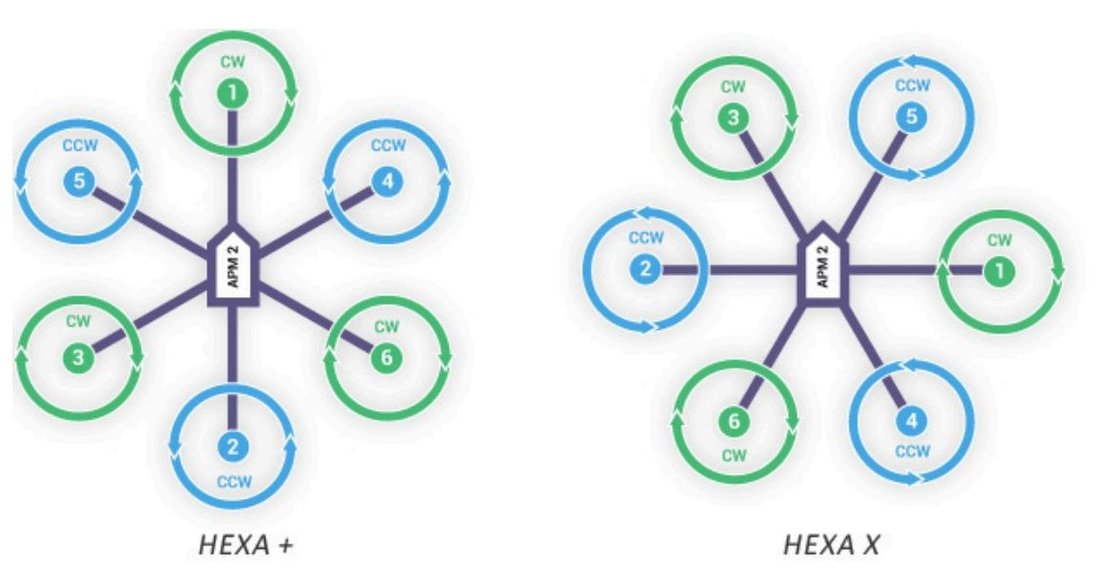
\includegraphics[width=10cm]{img/raspored.jpg}
\caption{Raspored motora heksakoptera\protect\footnotemark}
\label{fig:rasporedMotora}
\end{figure}
\footnotetext{Izvor: \url{http://www.arducopter.co.uk/uploads/6/7/0/2/6702064/1322957_orig.jpg}}
\citet{Zilic}  navodi  da su  prednosti  ove konfiguracije smanjenje dimenzija letjelica i nešto lakša konstrukcija što olakšava transport, a glavni nedostatak je smanjenje efikasnosti rada motora koja pada i do 20\% u odnosu na istu konfiguraciju  elektroničkih  komponenti  postavljenih  kao  standardni  oktakopter.  Osnovni elementi  multirotora  su  motori,  propeleri, upravljač leta,  baterija  i  konstrukcija  koja  sve  to povezuje   u   cjelinu   popularno   nazvan   okvir   \engl{frame}.  Za  multirotore  poboljšanih karakteristika koriste se motori bez četkica gdje su namotaji u središtu motora i imaju ulogu statora, a permanentni magneti su smješteni po obodu motora i imaju ulogu rotora. Glavna odlika ovih motora je pouzdan rad, jak okretni moment i velika brzina odaziva na promjenu broja okretaja motora. Ova zadnja karakteristika je ključni element za upravljanje multirotorom jer se upravljanje svodi na brze promjene broja okretaja motora.\\
Da bi multirotor uopće mogao funkcionirati i biti upravljiv mora imati upravljač leta. To je elektronski uređaj koji u sebi ima ugrađen elektronski kompas, žiroskop, akcelerometar (mjerač ubrzanja) i često barometar. Svaki bolji upravljač ima i GPS \engl{Global Positioning System} modul za očitavanja položaja. Obrađujući podatke od navedenih senzora upravljač šalje signale pojedinim motorima da smanje ili povećaju broj okretaja te na taj način održava stabilan let  multirotora.  Mnogi upravljači imaju mogućnost priključka vanjskog senzora  (npr.~sonar), koji daje podatak o udaljenosti od neke prepreke. \citep{Zilic}\\
Svi navedeni dijelovi multirotora smještaju se u konstrukciju. Pravilno je držati uravnoteženost multirotora po svim osima. Što je multirotor uravnoteženiji to će motori koristiti manje energije za upravljanje i stabilizaciju pa će cijela letjelica biti efikasnija. Multirotori su u mogućnosti izvoditi programirani let. To znači da se putem programa unaprijed odrede točke na koje treba doći sa definiranom visinom i brzinom između točaka. Bolju preciznost održavanja visine omogućava upravljač koji, pored  ostalih  senzora, ima i  barometar koji mu omogućuje letenje na  točno zadanoj  visini. \citep{Zilic}\\
\subsection{Petlje upravljanja}
Što se tiče samog upravljanja drona, odnosno praćenja trajektorije potrebne su dvije petlje. Unutarnja upravljačka petlja, odnosno prije spomenuti upravljač leta, upravlja visinom leta te nagibima multirotora. Ulazi u unutarnju petlju mogu se podijeliti na dva dijela --- na dio koji određuje zadatak \engl{task}, te na informacije koje daju senzori. Dijagram kontrole prikazan je slikom \ref{fig:dijagramKontrola}
\begin{figure}[htb]
\centering
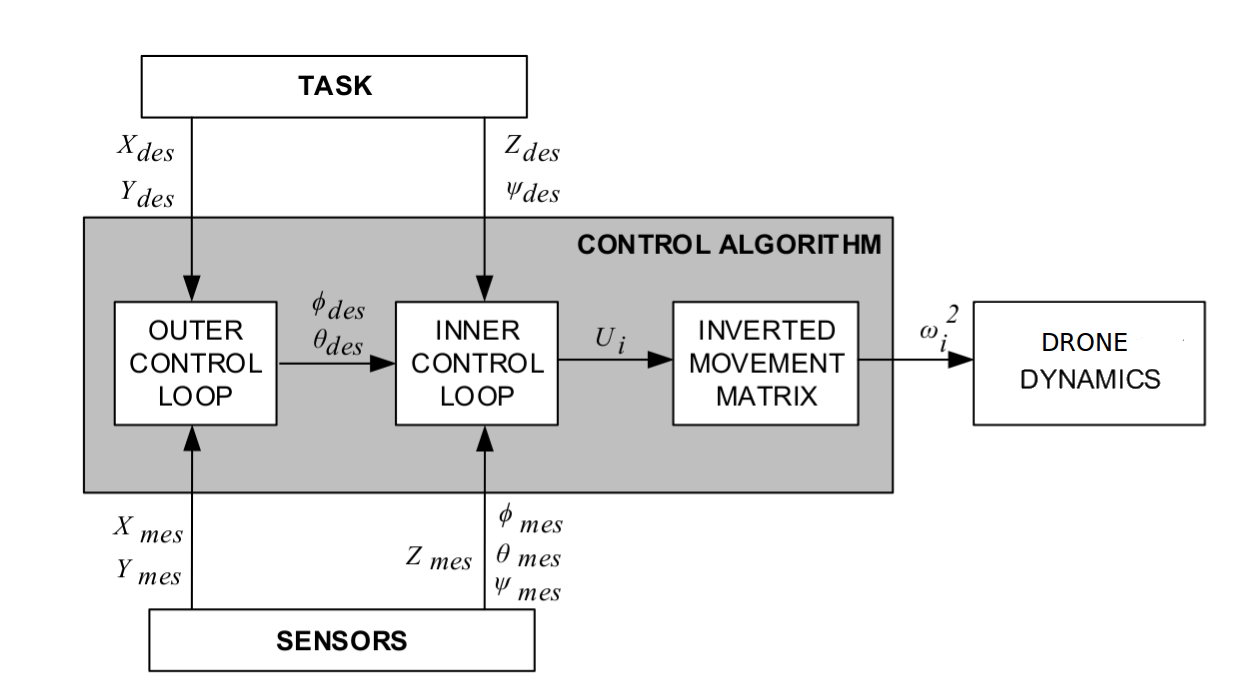
\includegraphics[width=14cm]{img/control_loop.png}
\caption{Dijagram kontrole drona}
\label{fig:dijagramKontrola}
\end{figure}
Varijable koje određuju zadatak su željena nadmorska visina i kut zavrtanja \engl{yaw} drona treba postići te željeni kutovi valjanja \engl{roll} i nagibanja \engl{pitch} koji se izračunavaju u vanjskoj upravljačkoj petlji. Senzori daju mjerenu nadmorsku visinu, kut valjanja \engl{roll}, kut nagiba \engl{pitch} i kut zavrtanja \engl {yaw}. Unutarnja izlazna petlja sadrži četiri upravljačke varijable. S informacijama iz senzora i dobrog algoritma kontrolera leta kontrola drona je bolja.
Vanjska upravljačka petlja je potrebna jer je dron u podređenom sustavu i nije moguće izravno kontrolirati sve motore na dronu. Kao što je već rečeno, unutarnja petlja izravno kontrolira motore, zadavajući tri kuta i nadmorsku visinu. Za indirektno kontroliranje $X_E$ i $Y_E$ položaja koristi se vanjska petlja. Vanjska upravljačka petlja, kao svoje izlaze, daje željeni kut valjanja \engl{roll} i nagibanja \engl{pitch} koji se prosljeđuju unutarnjoj petlji za definiranje željenog položaja $X_E$ i $Y_E$. Vanjska upravljačka petlja je superiorna unutrašnjoj upravljačkoj petlji.
Za dobro upravljanje dronom potrebno je poznavati i matematički model.


\section{Teoretski dio}\label{sec:SimulacijskiDio}
Svrha ovog poglavlja je preko matematičkih jednadžbi opisati dinamičko ponašanje heksakoptera koje se koriste za projektiranje, preko odgovarajućih metoda, kontrolera  za stabilizaciju i kontroler za slijeđenje željene trajektorije. Izabran je heksakopter jer je on korišten u eksperimentalnom dijelu. Heksakopter se sastoji od šest rotora koji su smješteni na vrhovima šesterokuta koji su jednako udaljeni od centra mase, odnosno od tri para suprotno rotirajućih i fiksno dijagonalno postavljenih elisa.  Kontrolira se podešavanjem kutne brzine rotora (vrtnja samo u jednom smjeru) koji se okreću pomoću električnih motora. To uvelike olakšava postupke projektiranja. Povećanjem broja rotora povećava se nosivot i olakšava upravljanje kod kvara jednog od motora. Pretpostavlja se da je letjelica kruto tijelo tako da se dinamika može izvesti diferencijalnim jednadžbama iz Newton-Euler i Euler-Lagrange jednadžbi. Eulerov kut parametrizacije trodimenzionalnih rotacija sadrži singularne točke u koordinatnom prostoru koji mogu uzrokovati pogreške i u dinamičkom modelu i kontroli. Da bi se spriječio singularitet, rotacija letjelice je parametrizirana kvaternionima. Ovom parametrizacijom u obzir je uzeta linearnost kvaterniona, njihova stabilnost i učinkovitost (potrebno manje vremena za obradu tijekom simulacije). Vrijedi napomenuti da su kvaternioni i Eulerovi kutevi povezani. Robusno matematičko modeliranje zajedno s učinkovitim upravljanjem osigurava lagan i siguran let. \citep{MathematicalModeling}
\begin{figure}[htb]
\centering
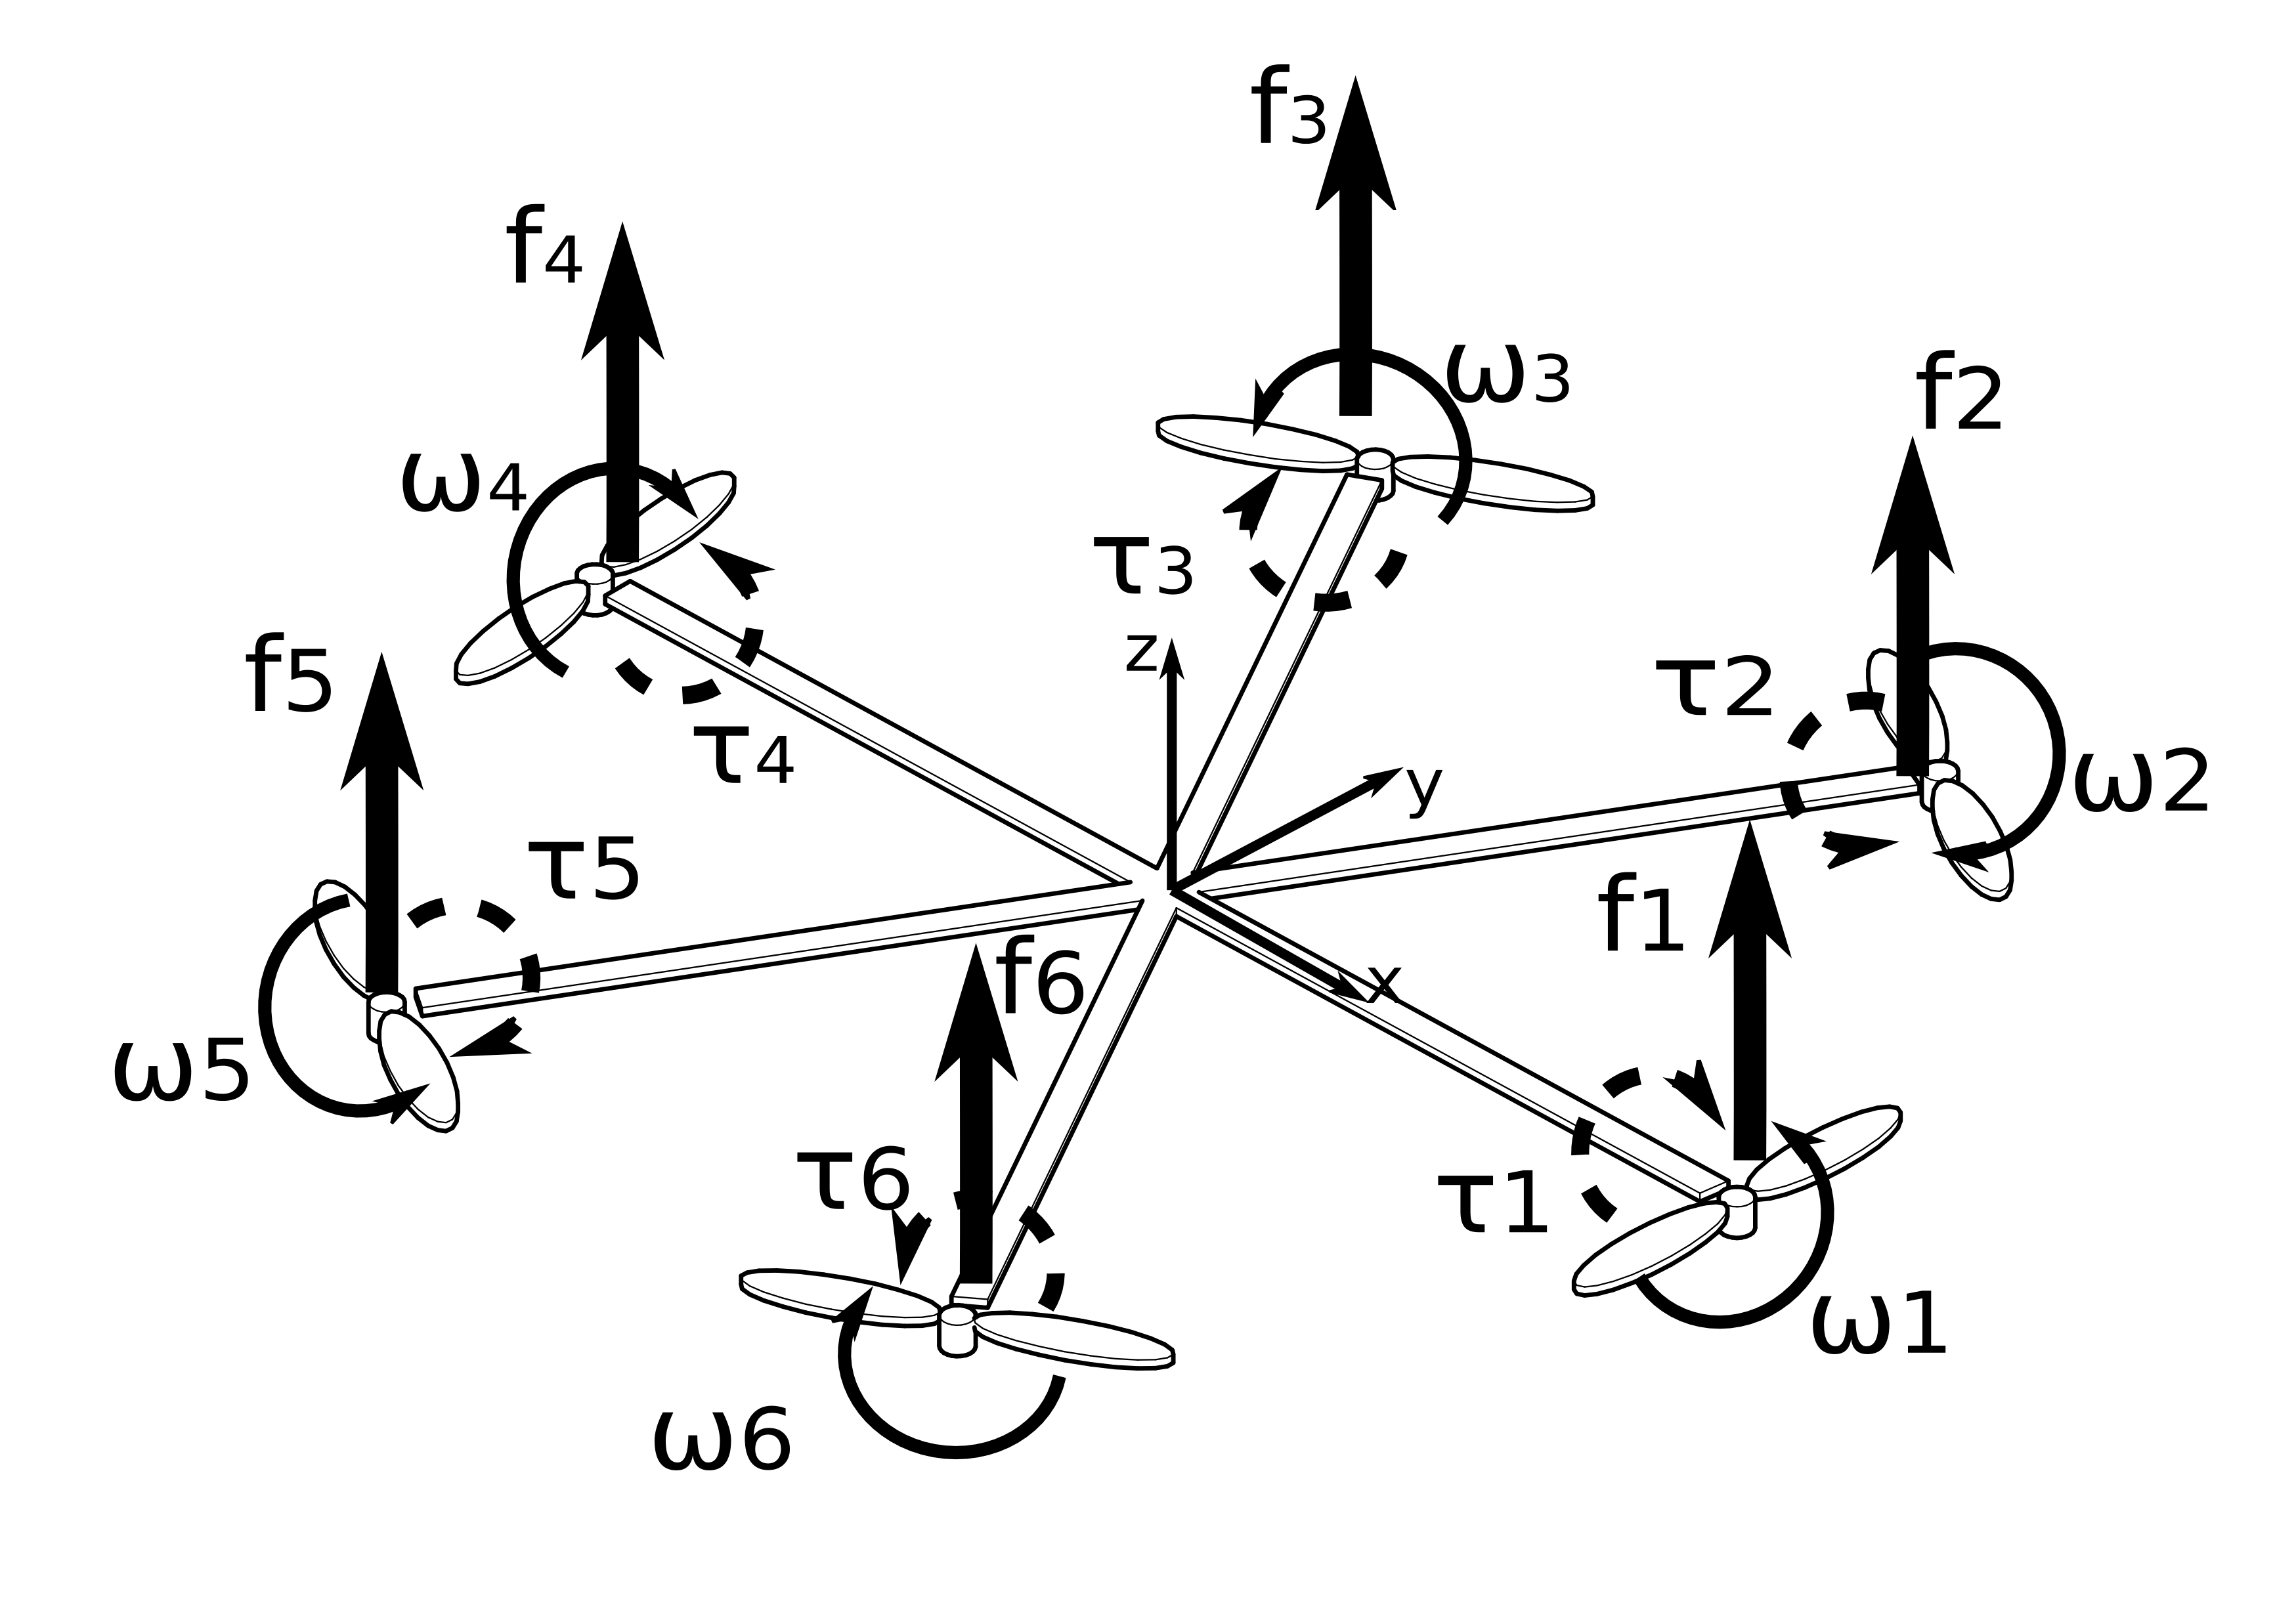
\includegraphics[width=8cm]{img/model_hexcopter.png}
\caption{Model heksakoptera\protect\footnotemark}
\label{fig:model}
\end{figure}
\footnotetext{Izvor: \url{https://www.researchgate.net/profile/V_Artale/publication/269073664/figure/fig1/AS:392210915840007@1470521777957/The-body-frame-of-an-hexacopter.ppm}}

\subsection{Eulerovi kutovi}\label{sec:Euler}
Shematski prikaz heksakoptera prikazan je na slici~\ref{fig:model}. Da bi opisali gibanje heksakoptera potrebna su dva referentna sustava:\begin{itemize}
\item nepomični globalni koordinatni sustav,
\item pokretni lokalni koordinatni sustav heksakoptera.
\end{itemize}
Nultočka nepomičnog globalnog koordinatnog sustava postavljena je u jednoj točci (npr.~kut prostorije) te su osi tog koordinatnog sustava ortogonalne te raspoređene prema \emph{desnoj orijentaciji} u kojem je apsolutna linearna pozicija izražena kao $(\mathbf{x,y,z})$. Za određivanje orijentacije letjelice potrebno je definirati pokretni koordinatni sustav $(X_p,Y_p,Z_p)$ koji se giba zajedno s heksakopterom, a centar tog koordinatnog sustava nalazi se u centru mase heksakoptera i orijentirani je kao na slici~\ref{fig:model}. Smjer ortonormiranih vektora $X_p,Y_p,Z_p$ u svakom se trenutku može izraziti u odnosu prema nepomičnom globalnom koordinatnom sustavu. Slijed rotacija oko ortonormiranih vektora pomičnog koordinatnog sustava predstavljen je tzv.~Eulerovim kutovima --- valjanje \engl{roll} $\phi$, nagibanje \engl{pitch} $\theta$ i zavrtanje \engl{yaw} $\psi$. Radi jednostavnosti označimo pokretni vektor pozicije i Eulerove kutove s $\xi = [x ~y ~z]^T$ i $\eta = [\phi ~\theta ~\psi]^T$. Transformaciju iz  lokalnog u globalni koordinatni sustav realizirana je s dobro znanom matricom rotacije \textbf{R} (izraz \ref{eq:matRot}) koja je ortogonalna.
\begin{equation}
	\begin{bmatrix}
	\cos\theta\cos\psi & \cos\psi\sin\theta\sin\phi-\cos\phi\sin\psi & \cos\phi\cos\psi\sin\theta+\sin\phi\sin\psi \\
	\cos\theta\sin\psi & \cos\phi\sin\psi+\sin\theta\sin\phi\sin\psi & \cos\phi\sin\theta\sin\psi-\cos\psi\sin\phi \\
	-\sin\theta & \cos\theta\sin\phi & \cos\theta\cos\phi \\
	\end{bmatrix}
	\label{eq:matRot}
\end{equation}
Kao posljedica, transformacijska matrica iz globalnog u lokalni koordinatni sustav je $\mathbf{R^{-1} = R^{T}}$. Matrica transformacije kutnih brzina iz lokalnog u globalni sustav je prikazana izrazom~\ref{eq:matBrzina}\footnote{Napomena: $\sec x = \frac{1}{\cos x}$}:
\begin{equation}
	\mathbf{W^{-1}_\eta} =
	\begin{bmatrix}
	1 & \sin\phi\tan\theta & \cos\phi\tan\theta \\
	0 & \cos\phi & -\sin\phi \\
	0 & \sec\theta\sin\phi & \cos\phi\sec\theta \\
	\end{bmatrix}
	\label{eq:matBrzina}
\end{equation}
Tada su zakoni transformacije~\ref{eq:v} i~\ref{eq:eta} gdje je $\nu$ definiran kao vektor $\nu=[\mathbf{p ~q ~r}]^T$.
\begin{align}
\nu&=\mathbf{W_\eta}\dot{\eta},\label{eq:v}\\
\dot{\eta}&=\mathbf{W^{-1}_\eta}\nu.\label{eq:eta}
\end{align}
Važno je uočiti da se $\mathbf{W^{-1}_\eta}$ može definirati samo i samo ako $\theta \neq \pi/2+k\pi, (k \in Z)$. Ovaj efekt kod Eulerovih formula je ograničenje \engl{gimbal lock}, tipična situacija kod koje se gubi stupanj slobode. Uzimanjem drugačijeg prikaza orijentacije u prostoru identificiranog s četiri parametra, poznatijim kao kvaternioni čija je generalna struktura objašnjena u poglavlju~\ref{sec:Kvaternioni} rješava se taj problem. Prednost kvarteniona ne leži samo u nepostojanju singulariteta nego i kod jednostavnosti izračuna, što će biti kasnije objašnjeno.

\subsection{Kvaternioni}\label{sec:Kvaternioni}
U poglavlju~\ref{sec:Euler} može se primijetiti da bi rotacija krutog tijela u prostoru mogla biti predstavljena preko Eulerovih kutova, međutim zbog singularnosti transformacijskih zakona potrebno je koristiti novu parametrizaciju kvaternionima. Kvaternioni se obično koriste u razvoju računalnih igara i u 3D virtualnom svijetu, ali također i kao metoda za pozicioniranje krutog tijela u trodimenzionalnom prostoru. Kvaternioni se temelje na Eulerovom teoremu rotacije koji definira da svaki pomak krutog tijela gdje točka ostaje nepromijenjena je ekvivalentna rotaciji. Dakle, ako je $\alpha$ kut rotacije oko jediničnog vektora $\mathbf{u} = (u_1, ~u_2, ~u_3)$, moguće je definirati kvaternion $\mathbf{q} = [q_0 ~q_1 ~q_2 ~q_3]^T$, gdje su $q_0 = \cos(\alpha/2), ~q_1 = \sin(\alpha/2)u_1, ~q_2 = \sin(\alpha/2)u_2, ~q_3 = \sin(\alpha/2)u_3$, koji definira tri dimenzije rotacije. Kvaternioni uvijek moraju zadovoljavati jednadžbu ograničenosti (\ref{eq:normalniUvjet}) koja je poznatija kao normalni uvjet. 
\begin{align}
q^2_0+q^2_1+q^2_2+q^2_3=1 \label{eq:normalniUvjet}
\end{align}
Za razliku od Eulerovih kutova kvaternionske rotacije ne zahtijevaju skup unaprijed definiranih rotacijskih osi jer jedna os se konstantno može mijenjati. Zbog svojstva ove metode da orijentacija ima samo jednu os rotacije, stupanj slobode se ne može izgubiti, odnosno ne postoji ograničenje. Transformacija translacijskih brzina gledano iz globalnog sustava može se izraziti preko \ref{eq:transBrzina} gdje je $\mathbf{Q}$ matrica~\ref{eq:matQ}.
\begin{align}
\xi=\mathbf{Q\xi_B} \label{eq:transBrzina}
\end{align}
\begin{equation}
	\mathbf{Q} =
	\begin{bmatrix}
	q^2_0+q^2_1-q^2_2-q^2_3 & 2(q_1q_2-q_0q_3) & 2(q_0q_2+q_1q_3) \\
	2(q_1q_2+q_0q_3) & q^2_0-q^2_1+q^2_2-q^2_3 & 2(q_2q_3-q_0q_1) \\
	2(q_1q_3-q_0q_2) & 2(q_0q_1+q_2q_3) & q^2_0-q^2_1-q^2_2+q^2_3 \\
	\end{bmatrix}
	\label{eq:matQ}
\end{equation}
Kao matrica $\mathbf{R}$ i matrica $\mathbf{Q}$ je ortogonalna, pa vrijedi također $\mathbf{Q^{-1} = Q^{T}}$. Kutna brzina, uključujući transformaciju, može se izraziti kao $\mathbf{\dot{q}}=\mathbf{S}~\nu$ gdje matrica $\mathbf{S}$ ovisi o kvartenijskim komponentama prikazanim~\ref{eq:matS}.
\begin{equation}
	\mathbf{S} = \frac{1}{2}
	\begin{bmatrix}
	-q_1 & -q_2 & -q_3 \\
	q_0 & -q_3 & q_2 \\
	q_3 & q_0 & -q_1 \\
	-q_2 & q_1 & q_0 \\
	\end{bmatrix}
	\label{eq:matS}
\end{equation}
Zaključak, korist korištenjem kvaterniona je dvostruka: \begin{enumerate}
\item dohvaćanje svih pozicija (i onih kritičnih),
\item zahvaljujući linearnosti koeficijenata transformacijske matrice, izračun putem kvaterniona je učinkovitiji i stabilniji u odnosu s tradicionalnim izračunom.
\end{enumerate}

\subsection{Matematički model hexkoptera}
U ovom odjeljku prikazan je matematički model heksakoptera.  Dinamika šest električnih motora je relativno brza pa će se stoga zanemariti. Cilj je odrediti matematičke jednadžbe koje opisuju dinamičko ponašanje heksakoptera pomoću generalizacije opisane sa slikom~\ref{fig:model} i poglavljem~\ref{sec:SimulacijskiDio}. Mogu se primijeniti Newton-Euler i Euler-Lagrange jednadžbe.\\

\subsubsection{Newton-Euler jednadžbe}
Gibanje krutog tijela može se razložiti na translacijsku i rotacijsku komponentu. Stoga, kako bi se opisala dinamika heksakoptera, pretpostavka je da je letjelica kruto tijelo pa se za izračun koriste Newton-Eulerove jednadžbe koje reguliraju linearno i kružno gibanje. Sila koja djeluje na heksakopter prikazana je \ref{eq:Sila}, gdje se pretpostavlja da je $m$ konstantna masa.
\begin{align}
\mathbf{F}&=\mathbf{\frac{d(m~v_B)}{dt}+\nu\times (m~v_B)} \label{eq:Sila}
\end{align}
Svaki rotor $i$ ima kutnu brzinu $\omega_i$ koja stvara silu $\mathbf{f_i}=k[0 ~0 ~\omega^2_i]$, gdje je $k$ konstanta potiska, dakle ukupan potisak \engl{thrust} $\mathbf{T_B}$ dan je s \ref{eq:TB} i \ref{eq:Tsila}
\begin{align}
\centering
\mathbf{T_B}&=\mathbf{[0 ~0 ~T]^T} \label{eq:TB} \\
\mathbf{T}&=\sum_{i=1}^{6}f_i=k\sum_{i=1}^{6}\omega_i \label{eq:Tsila}
\end{align}
Ukupan potisak zajedno s gravitacijom predstavlja ukupnu silu (izraz \ref{eq:Fukupna}) koja djeluje na heksakopter.
\begin{align}
\mathbf{F}&=\mathbf{Q^TF_g+T_B} \label{eq:Fukupna}
\end{align}
Kao posljedica, translacijska komponenta gibanja u lokalnom sustavu je \ref{eq:Flokalni}.
\begin{align}
m~\mathbf{\dot{v_B}+\nu\times (m~v_b)}&=\mathbf{Q^TF_g+T_B} \label{eq:Flokalni}
\end{align}
Da bi dobili istu jednadžbu u globalnom sustavu, potrebno je primijetiti da je centrifugalna sila poništena jer se globalni sustav ne rotira pa tako prethodna jednadžba postaje~\ref{eq:Fglobalni}
\begin{align}
m~\mathbf{\ddot{\xi}}&=\mathbf{F_g+Q~T_B} \label{eq:Fglobalni}
\end{align}
Nadalje, neka je $\mathbf{I}$ matrica inercija. Heksakopter ima simetričnu strukturu s obzirom na $X_b$-os, $Y_b$-os i $Z_b$-os, stoga je matrica inercija jedinična $\mathbf{I}=diag(\mathbf{I_{xx}, I_{yy}, I_{zz}})$. Kako ukupni vanjski moment $\mathbf{M}$ djeluje, uzimajući u obzir brzinu promjene kutnog momenta  $\mathbf{H=I\nu}$ tada je moment koji djeluje na heksakopter izražen s~\ref{eq:MomentHex}.
\begin{align}
\mathbf{M}&=\mathbf{\frac{d(I~\nu)}{dt}+\nu\times(I~\nu)} \label{eq:MomentHex}
\end{align}
Kutna brzina i akceleracija rotora stvaraju okretni moment prikazan \ref{eq:Torque} oko osi rotora, gdje je $b$ konstanta otpora tereta te gdje je $I_{M_i}$ moment inercije rotora $i$.
\begin{align}
\tau_{M_i}&=b~\omega^2_i+I_{M_i}~\dot{\omega_i} \label{eq:Torque}
\end{align}
Iz geometrijske strukture heksakoptera i od komponenata $\mathbf{f_i}$ i $\mathbf{\tau_{M_i}}$ u lokalnom koordinatnom sustavu moguće je dobiti informaciju o momentima \emph{roll, pitch i yaw} preko~\ref{eq:matTau}.
\begin{equation}
	\begin{bmatrix}
	\tau_{\phi} \\
	\tau_{\theta} \\
	\tau_{\psi}
	\end{bmatrix}
	=
	\begin{bmatrix}
	\frac{3}{4}kl(\omega^2_2+\omega^2_3-\omega^2_5-\omega^2_6) \\
	kl(-\omega^2_1-\frac{\omega^2_2}{4}+\frac{\omega^2_3}{4}+\omega^2_4+\frac{\omega^2_5}{4}-\frac{\omega^2_6}{4}) \\
	b(-\omega^2_1+\omega^2_2-\omega^2_3+\omega^2_4-\omega^2_5+\omega^2_6)+I_M(\dot{\omega^2_1}+\dot{\omega^2_2}+\dot{\omega^2_3}+\dot{\omega^2_4}+\dot{\omega^2_5}+\dot{\omega^2_6})
	\end{bmatrix}
	\label{eq:matTau}
\end{equation}
Ovdje je $l$ udaljenost između rotora i središta mase heksakoptera, a $\dot{x}_{\omega_i}$ predstavlja vremensku derivaciju $\omega_i(t)$\footnote{Vremenska derivacija: $\frac{d\omega_i(t)}{dt}$}. Nadalje, jednadžba koja određuje dinamiku rotacije može se zapisati kao \ref{eq:rotDin} gdje $\mathbf{\Gamma}$ predstavlja žiroskopske sile i $\mathbf{\tau_B}$ vanjski okretni moment.
\begin{align}
\mathbf{I~\dot{\nu}+\nu\times(I~\nu)}+\Gamma&=\mathbf{\tau_B} \label{eq:rotDin}
\end{align}
Nakon kratkog izračuna dobije se \ref{eq:vDot} u kojoj je 
\begin{align}
\omega_{\Gamma} &= \omega_1-\omega_2+\omega_3-\omega_4+\omega_5-\omega_6 \label{eq:omegaV}
\end{align}
\begin{equation}
	\dot{\nu} = \mathbf{I^{-1}} \Bigg(
	\begin{bmatrix}
	p \\
	q \\
	r
	\end{bmatrix}
	\times
	\begin{bmatrix}
	I_xx~p \\
	I_yy~q \\
	I_zz~r
	\end{bmatrix}
	-\mathbf{I_r}
	\begin{bmatrix}
	p \\
	q \\
	r
	\end{bmatrix}
	\times
	\begin{bmatrix}
	0 \\
	0 \\
	1
	\end{bmatrix}
	\mathbf{\omega_{\Gamma}}+\tau
	\Bigg)
	\label{eq:vDot}
\end{equation}
Inače jednadžba \ref{eq:vDot} može se pisati kao \ref{eq:vDot2}
\begin{equation}
	\begin{bmatrix}
	\dot{p} \\
	\dot{q} \\
	\dot{r}
	\end{bmatrix}
	=
	\begin{bmatrix}
	(I_{yy}-I_{zz})~q~r/I_{xx} \\
	(I_{zz}-I_{xx})~p~r/I_{yy} \\
	(I_{xx}-I_{yy})~p~q/I_{zz}
	\end{bmatrix}
	-\mathbf{I_r}
	\begin{bmatrix}
	q/I_{xx} \\
	-p/I_{yy} \\
	0
	\end{bmatrix}
	\mathbf{\omega_{\Gamma}}+
	\begin{bmatrix}
	\tau_{\phi}/I_{xx} \\
	\tau_{\theta}/I_{yy} \\
	\tau_{\psi}/I_{zz}
	\end{bmatrix}
	\label{eq:vDot2}
\end{equation}
Konačno, nakon određivanja kutne brzine lako se odredi i kutno ubrzanje u globalnom koordinatnom sustavu preko izraza \ref{eq:angularAcceleration}.
\begin{align}
\mathbf{\ddot{q}}&=\mathbf{\frac{d(S~\nu)}{dt}} \label{eq:angularAcceleration}
\end{align}

\subsubsection{Euler-Lagrange jednadžbe}
Newton-Eulerova forma se temelji na ravnoteži sile i momenata. Alternativa tim jednadžbama, koristeći pristup temeljen na sačuvanje energije, su Euler-Lagrangeove jednadžbe. Prije svega, definicija Lagrangiana je izražena \ref{eq:Lagrangian} gdje je $E_t = (m/2)\mathbf{\dot{\xi}^T\dot{\xi}}$ translacijska kinetička energija, $E_r = (1/2)\mathbf{\nu^T~I~\nu}$ je kutna energija te $E_p=m~g~z$ je potencijalna energija gdje je $z$ visina heksakoptera.
\begin{align}
\mathcal{L}&=E_t+E_r-E_p \label{eq:Lagrangian}
\end{align}
Dinamički model letjelice dobiva se iz \ref{eq:dinModL} gdje $\bf f$ predstavlja vanjske sile koje utječu na potisak $\bf T_B$, $\tau=4\bf {S \tau_B}$ je generalizirani okretni moment i $\mathbf{w=\left[ \xi^T, q^T \right]}$ su Lagrangianove koordinate.
\begin{equation}
{d\over dt}\left({\partial {\cal L}\over \partial\dot{{\bf w}}}\right)-{\partial {\cal L}\over \partial{\bf w}}= \begin{bmatrix}\bf f \\ \bf\tau \end{bmatrix} \label{eq:dinModL}
\end{equation}
Budući da kinetička energija ne sadrži kombinaciju $\dot{\xi}$ i $\dot{\bf q}$, translacijska i rotacijska dinamika se mogu razmatrati zasebno. Translacijsko gibanje može se izraziti jednadžbom \ref{eq:transGiba} koja je jednaka kao \ref{eq:Flokalni}.
\begin{equation}
m\ddot{{\ \xi}}-{\bf F}_{g}={\bf f}={\bf Q\ T}_{B} \label{eq:transGiba}
\end{equation}
Potrebno je da se definira rotacijsko gibanje s generaliziranim koordinatama, ovdje brzina $\xi$ mora biti opisana kvaternionom $\bf q$.\\
Vidljivo je da se $\xi$ ne može dobiti iz \ref{eq:transBrzina} direktno, jer matrica $\bf S$ nije kvadratna, pa nije ni invertibilna. No produkt između $\bf S$ i njegove transponirane matrice je \ref{eq:productSt_S} gdje je $\cal I$ jedinična matrica dimenzije $3\times3$. 
\begin{equation}
{\bf S}^{T}{\bf S}={1\over 4}{\cal I} \label{eq:productSt_S}
\end{equation}
Dakle, lijevim množenjem s $\mathbf{S_T}$ izraza \ref{eq:productSt_S} dolazi se do \ref{eq:lijevoMnozenje} iz kojeg se dobije brzina \ref{eq:brzinaL}.
\begin{align}
{\bf S}^{T}\dot{{\bf q}}&={\bf S}^{T}{\bf S}{\ \nu}={1\over 4}{\cal I}{\ \nu} \label{eq:lijevoMnozenje} \\
{\ \nu}&=4{\bf S}^{T}\dot{{\bf q}} \label{eq:brzinaL}
\end{align}
Definiranjem \ref{eq:defJ}, kutna energija može se izraziti s \ref{eq:kutnaE}.
\begin{align}
{\bf J}&={\bf S\ I} \ {\bf S}^{T} \label{eq:defJ} \\
E_{r}&={1\over 2}{\ \nu}^{T}{\bf I}{\ \nu}=8\dot{{\ q}}^{T}{\bf J}\dot{{\ q}} \label{eq:kutnaE}
\end{align}
Sada je moguće napisati rotacijsku jednadžbu (\ref{eq:rotJedna}) preko kvaterniona $\bf q$. 
\begin{align}
8\bigg[2{\bf J}\ddot{{\bf q}}+2{d{\bf J}\over dt}\dot{q}-{\partial\over \partial {\bf q}}(\dot{q}^{T}{\bf J}\dot{q})\bigg]&={\ \tau} \label{eq:rotJedna}
\end{align}
Stoga je matematički model koji opisuje heksakopter izražen Euler-Lagrange formom prikazan \ref{eq:matModelL}.
\begin{align}
\ddot{{\bf q}}&={1\over 2}{\bf J}^{-1}\bigg[{1\over 8}{ \tau}-2{d{\bf J}\over dt}\dot{{\ q}}+{\partial\over \partial_{{\bf q}}}(\dot{q}^{T}{\bf J}\dot{q})\bigg] \label{eq:matModelL}
\end{align}
Može se uočiti da su ovi izrazi ekvivalentni izrazima \ref{eq:vDot} i \ref{eq:angularAcceleration}.

\subsection{Sinteza sustava upravljanja}
U ovom poglavlju projektira se regulator za slijeđenje željene trajektorije. Koriste se kvaternioni jer smanjuju nestabilnost te ubrzavaju numerički račun. Jednostavan i lako izvediv način upravljana, tj. njegove stabilizacije, realiziran je proporcionalno-derivacijskim (PD) regulatorom. PD regulatoru dodaje se integralna komponenta s ciljem smanjenja efekta fluktuacije \engl{fluctuations} heksakoptera koje su uzrokovane vanjskim poremećajima.
U izrazu \ref{eq:matQ} prikazana je kontrola leta heksakoptera. Konkretno, razvijena je jednostavna heuristička metoda za slijeđenje željene trajektorije. \\
Generalno, PID regulator koji prati referencu ima formu \ref{eq:PIDe} i \ref{eq:PIDu} gdje je $u(t)$ upravljački ulaz i $e(t)$ predstavlja pogrešku između reference $r_d(t)$ i trenutne pozicije $x(t)$.
\begin{align}
e(t) &= x_d(t) - x(t) \label{eq:PIDe} \\
u(t) &= K_p~e(t) + K_I \int_0^t {\mathrm{e(s)}\,\mathrm{d}s} + K_D {d\over dt} e(t) \label{eq:PIDu}
\end{align}
Koeficijenti $K_p, K_I, K_D$ predstavljaju parametre za proporcionalni, integracijski te derivacijski član PID regulatora. PID regulator se primjenjuje na sustav, prikazan \ref{eq:Torque} i \ref{eq:rotDin}, koji opisuje kretanje letjelice, tj.~njezin položaj. Može se pisati:
\begin{align}
d_x &= K_{x,P}~(x_d-x)+K_{x,D}~(\dot{x}_d-\dot{x})+K_{x,I} \int_0^t {\mathrm{(x_d-x)}\,\mathrm{d}s} \label{eq:PIDdy} \\
d_y &= K_{y,P}~(y_d-y)+K_{y,D}~(\dot{y}_d-\dot{y})+K_{y,I} \int_0^t {\mathrm{(y_d-y)}\,\mathrm{d}s} \label{eq:PIDdy} \\
d_z &= K_{z,P}~(z_d-z)+K_{z,D}~(\dot{z}_d-\dot{z})+K_{z,I} \int_0^t {\mathrm{(z_d-z)}\,\mathrm{d}s} \label{eq:PIDdy}
\end{align}
\subsubsection{Kvaternioni}
Razlika između klasičnih pristupa linearizacije, poput Lyapunove linearizacije ili linearizacije najmanjim kvadratima, i pristupa putem kvaterniona je u kvaternionskoj pogrešci $q_e$ --- ona je definirana kao razlika između željene orijentacije i trenutne izraženih preko kvaterniona. To dovodi do izraza \ref{eq:PIDqe1}-\ref{eq:PIDqe4} gdje je $\bf q_d$ kvaternion koji odgovara željenoj \emph{yaw} orijentaciji te kvaternion $\bf q$ koji odgovara trenutnoj orijentaciji. 
\begin{align}
q_{e,1} &= -q_{d,0}q_1 -q_{d,3}q_2 + q_{d,2}q_3 + q_{d,1}q_0 \label{eq:PIDqe1} \\
q_{e,2} &= q_{d,3}q_1 -q_{d,0}q_2 - q_{d,1}q_3 + q_{d,2}q_0 \label{eq:PIDqe2} \\
q_{e,3} &= -q_{d,2}q_1 +q_{d,1}q_2 - q_{d,0}q_3 + q_{d,3}q_0 \label{eq:PIDqe3} \\
q_{e,4} &= q_{d,1}q_1 +q_{d,2}q_2 + q_{d,3}q_3 + q_{d,0}q_0 \label{eq:PIDqe4}
\end{align}
Tada se komponente momenta $\tau_{\phi}, \tau_{\theta},\tau_{\psi}$ mogu se zapisati kao \ref{eq:tauPhi}-\ref{eq:tauPsi}.
\begin{align}
\tau_{\phi} &= (K_{\phi,D}~p + K_{\phi,P}~q_{e,1}~q_{e,4})~I_{xx} \label{eq:tauPhi} \\
\tau_{\theta} &= (K_{\theta,D}~q + 2K_{\theta,P}~q_{e,2}~q_{e,4})~I_{yy} \label{eq:tauTheta} \\
\tau_{\psi} &= (K_{\psi,D}~r + 2K_{\psi,P}~q_{e,3}~q_{e,4})~I_{zz} \label{eq:tauPsi}
\end{align}
Točne kutne brzine rotora $\omega_i$, koje su također upravljački ulazi izvedene su izrazima \ref{eq:omega1}-\ref{eq:omega6} gdje $k$ označuje potisnu konstantu, $b$ označuje vučnu konstantu, a $l$ predstavlja udaljenost između rotora i centra mase heksakoptera.
\begin{align}
\omega^2_1 &= \frac{T}{6k} - \frac{2\tau_{\theta}}{5kl} - \frac{\tau_{\psi}}{10b} \label{eq:omega1} \\
\omega^2_2 &= \frac{T}{6k} + \frac{\tau_{\phi}}{3kl} -\frac{2\tau_{\theta}}{5kl} + \frac{\tau_{\psi}}{5b} \label{eq:omega2} \\
\omega^2_3 &= \frac{T}{6k} + \frac{\tau_{\phi}}{3kl} + \frac{2\tau_{\theta}}{5kl} - \frac{\tau_{\psi}}{5b} \label{eq:omega3} \\
\omega^2_4 &= \frac{T}{6k} + \frac{2\tau_{\theta}}{5kl} + \frac{\tau_{\psi}}{10b} \label{eq:omega4} \\
\omega^2_5 &= \frac{T}{6k} - \frac{\tau_{\phi}}{3kl} + \frac{2\tau_{\theta}}{5kl} - \frac{\tau_{\psi}}{5b} \label{eq:omega5} \\
\omega^2_6 &= \frac{T}{6k} - \frac{\tau_{\phi}}{3kl} -\frac{2\tau_{\theta}}{5kl} + \frac{\tau_{\psi}}{5b} \label{eq:omega6} 
\end{align}
Neka $\bf \ddot{\xi}, \dot{\xi}$ i $\bf q_3$ definiraju željenu trajektoriju. Koristeći izraze \ref{eq:Flokalni}-\ref{eq:vDot} i normalni uvjet \ref{eq:normalniUvjet} možemo izraziti $q_0$ (\ref{eq:q0}), $q_1$ (\ref{eq:q1}), $q_2$ (\ref{eq:q2}) i ukupni potisak $\bf T$ (\ref{eq:T}). 
\begin{align}
q_0 &= \sqrt{\frac{1}{2} + \frac{d_z+g}{2\sqrt{d^2_x+d^2_y+(d_z+g)^2}}-q^2_3} \label{eq:q0} \\
T &= \frac{m(d_z + g)}{2~(q^2_0 + q^2_3)-1} \label{eq:T} \\
q_1 &= \frac{m(d_z q_3 - d_y q_0)}{(q^2_0 + q^2_3)~2T} \label{eq:q1} \\
q_2 &= \frac{m(d_z q_0 - d_y q_3)}{(q^2_0 + q^2_3)~2T} \label{eq:q2}
\end{align}
Valja ponovo istaknuti da se heksakopterom upravlja podešavanjem brzina vrtnje propelera koji se pokreću elektromotorima. 

\subsubsection{Eulerovi kutevi}
Odnosno gledajući Eulerove kuteve jednadžbe akceleracija su \ref{eq:X}-\ref{eq:Z}, gdje su $\ddot{X}, \ddot{Y}, \ddot{Z}$ akceleracije u fiksnom koordinatnom sustavu, a $omega_{\Gamma}$ je izražena izrazom \ref{eq:omegaV}.
\begin{align}
\ddot{X} &= (\cos\psi \sin\theta \cos\phi + sin\psi \sin\phi)\frac{U_1}{m} \label{eq:X} \\
\ddot{Y} &= (\sin\psi \sin\theta \cos\phi - cos\psi \sin\phi)\frac{U_1}{m} \label{eq:Y} \\
\ddot{Z} &= -g + (\cos\theta \cos\phi)\frac{U_1}{m} \label{eq:Z} \\
\dot{p} &= \frac{I_{yy}-I_{zz}}{I_{xx}}qr - \frac{J_{TP}}{I_{xx}}q\omega_{\Gamma} + \frac{U_2}{I_{xx}} \label{eq:p} \\
\dot{q} &= \frac{I_{zz}-I_{xx}}{I_{yy}}pr - \frac{J_{TP}}{I_{yy}}p\omega_{\Gamma} + \frac{U_3}{I_{yy}} \label{eq:q} \\
\dot{r} &= \frac{I_{xx}-I_{yy}}{I_{zz}}pq  + \frac{U_4}{I_{zz}} \label{eq:r} \\
\end{align}
Izrazima \ref{eq:p}-\ref{eq:r} su prikazane kutne akceleracije u odnosu na fiksni koordinatni sustav. $J_{TP}$ je momenti inercije koji stvara propeler, dok je $\omega_{\Gamma}$ ukupna brzina propelera.  
Upravljačke veličine $U_1, U_2, U_3$ i $U_4$, prikazane izrazima \ref{eq:U1}-\ref{eq:U4}, su funkcije kvadratnih kutnih brzina gdje je $l$ udaljenost rotora od centra mase, $b$ je koeficijent potiska, a $d$ je koeficijent otpora.
\begin{align}
U_1 &= T = k~(\omega^2_1+\omega^2_2 +\omega^2_3+\omega^2_4+\omega^2_5+\omega^2_6) \label{eq:U1} \\
U_2 &= \tau_{\phi} =\frac{3}{4}kl(\omega^2_2+\omega^2_3-\omega^2_5-\omega^2_6) \label{eq:U2} \\
U_3 &= \tau_{\theta} = kl(-\omega^2_1-\frac{\omega^2_2}{4}+\frac{\omega^2_3}{4}+\omega^2_4+\frac{\omega^2_5}{4}-\frac{\omega^2_6}{4}) \label{eq:U3} \\
U_4 &= \tau_{\psi}= b(-\omega^2_1+\omega^2_2-\omega^2_3+\omega^2_4-\omega^2_5+\omega^2_6)+I_M(\dot{\omega^2_1}+\dot{\omega^2_2}+\dot{\omega^2_3}+\dot{\omega^2_4}+\dot{\omega^2_5}+\dot{\omega^2_6}) \label{eq:U4} 
\end{align}
Cilj stabilizacije je pronalaženje vrijednosti kutne brzine vrtnje propelera koji zadržava poziciju i orijentaciju. To se postiže preko inverzne kinematike, odnosno dinamike. No preko inverzne kinematike nije uvijek moguć izračun te nije uvijek jedinstvena. Dinamika heksakoptera mora biti pojednostavljena kako bi se mogla implementirati u algoritam upravljanja. Jednadžbe \ref{eq:X}-\ref{eq:r} mogu biti pojednostavljene uzimajući u obzir sljedeće pretpostavke:
\begin{itemize}
\item Kutni udjeli akceleraciji su vrlo složeni jer ovise o nekoliko parametara, od čega su većina vektorski produkti kutnih brzina. Imajući na umu da je heksakopter većinu vremena lebdi, takve male promjene u kutevima, odnosno njezini udjeli mogu se zanemariti.
\item Kutne akceleracije su povezane s promjenom kuteva u odnosu na lokalni koordinatni sustav drona. Transformacijska matrica $T$ definira odnos između brzina u odnosu na lokalni i globalni koordinatni sustav. Pošto je heksakopter blizu lebdenja $T$ je jedinična matrica, čineći tako jednadžbe kutnih ubrzanja jednakima u oba koordinatna sustava. 
\item Upravljački algoritam daje upravljačke signale motorima. S četiri upravljačke veličine nije moguće upravljati više od 4 stupnja slobode. Unutarnja petlja upravlja položajem i visinom, dok vanjska petlja upravlja pozicijom heksakoptera davajući referencu unutrašnjoj petlji.
\end{itemize}
Pojednostavljene jednadžbe dane su izrazima \ref{eq:Z2}-\ref{eq:kut3}.
\begin{align}
\ddot{Z} &= -g + (\cos\theta \cos\phi)\frac{U_1}{m} \label{eq:Z2} \\
\ddot{\phi} &= \frac{U_2}{I_{xx}} \label{eq:kut1} \\
\ddot{\theta} &= \frac{U_3}{I_{yy}} \label{eq:kut2} \\
\ddot{\psi} &= \frac{U_4}{I_{zz}} \label{eq:kut3} 
\end{align}
Ulazi u upravljački algoritam su podaci iz senzora (ili izračunati podaci iz dinamičkog modela) i referenca. Izlazi iz upravljačkog algoritma su kutne brzine šest propelera koje zadaju vrijednost napona koja preko pulsno širinske modulacije - \engl{pulse-width modulation - PWM} pokreće motore propelera. Heksakopter ne dopušta izravnu kontrolu svih stupnjeva slobode. Upravljanje X i Y pozicije postiže se indirektno kroz kontrolu kuteva valjanja \engl{roll} i nagibanja \engl{pitch} u vanjskoj petlji. 
Vanjska upravljačka petlja analizira podatke iz senzora i podatke o željenoj referenci te daje na izlazu vrijednosti za unutarnju upravljačku petlju koja zatim upravlja kutevima valjanja\engl{roll}, nagibanja \engl{pitch}
i zavrtanja \engl{yaw}. Unutarnja upravljačka petlja jezgra upravljačkog algoritma. Analizira podatke iz senzora i vanjske upravljačke petlje, te zajedno s željenim podacima o visini daje izlaz. Izlazi iz unutarnje upravljačke petlje su upravljačke varijable koje stabiliziraju heksakopter smanjujući pogrešku između reference i stvarnog položaja. Izrazima \ref{eq:U1}-\ref{eq:U4} izražavaju se upravljačke veličine za potrebna ubrzanja koje možemo pisati \ref{eq:omega1}-\ref{eq:omega6}. Za regulaciju tih ubrzanja koristi se PID regulator.


\section{Eksperimentalni dio}
U ovom poglavlju obrađen je eksperimentalni dio, tj.~provjera kvalitete projektiranog sustava upravljanja u laboratorijskim uvjetima. 
Cijena modernih bespilotnih letjelica doseže nekoliko desetaka tisuća kuna (postoje i skuplje) koje imaju ugrađeno mnogo senzora. U našem eksperimentalnom dijelu korištena je jeftinija verzija koja nema toliko senzora, pa su zbog tog korišteni dodatni vizualni senzori koji određuju položaj letjelice u prostoru. Korišten je heksakopter MJX X800 RC koji je prikazan na slici \ref{fig:MJX X800 RC} zajedno sa svojim kontrolerom (njegova cijena je oko 40\$). Također odabrano je programsko okruženje ROS preko kojeg će se cijeli sustav upravljati. 
\begin{figure}[htb]
\centering
\includegraphics[width=8cm]{img/heksakopterMJX.JPG}
\caption{Heksakopter MJX X800 RC sa svojim kontrolerom}
\label{fig:MJX X800 RC}
\end{figure}\\
Za potrebe eksperimenta potrebno je modificirati samog drona te odabrati način upravljanja preko računala. Postoje dva načina:
\begin{enumerate}
\item Slanjem upravljačkih signala putem radio signala\label{sec:radio}
\item Modificiranjem kontrolera, odnosno omogućiti slanje upravljačih signala preko kontrolera\label{sec:modifikacija}
\end{enumerate}
Na \ref{sec:radio}.~način potrebno je dobro poznavati kakve signale kontroler šalje dronu kako bi se ti signali mogli dronu slat preko \emph{wireless} kartice. Za ovakav postav potrebne su još Arduino, kamere te markeri na dronu. Pošto izabrani dron nema dostupni \emph{datasheet} jednostavnija verzija postava je  na \ref{sec:modifikacija}.~način. Za ovaj način upravljanje potrebno je:
\begin{itemize}
\item Heksakopter MJX X800 RC i njegova modifikacija (vidi \ref{sec:heksakopter})
\item Sustav kamera (vidi \ref{sec:kamera})
\item Kontroler i njegova modifikacija pomoću Arduina (vidi \ref{sec:kontroler})
\item Računalo s algoritmom upravljanja (vidi \ref{sec:algoritam})
\end{itemize}

\subsection{Heksakopter MJX X800 RC i njegova modifikacija}\label{sec:heksakopter}
Modifikacija heksakoptera je u smislu dodavanja markera za njegovo praćenje u sustavu globalne vizije. Potrebno je koristiti barem 3 markera kako ne bi izgubili podatke o svim orijentacijama. Zbog robusnosti i stabilnosti kao markeri korištene su infracrvene \engl{IR} svjetleće diode \engl{Light Emitting Diode - LED}. Korištene su svjetleće diode visoke snage i široke kutne vidljivosti, konkretno korištena je 3W svjetleća dioda koja ima \ang{120} kutne vidljivosti (prikazana slikom \ref{fig:LED}). \\
\begin{figure}[htb]
\centering
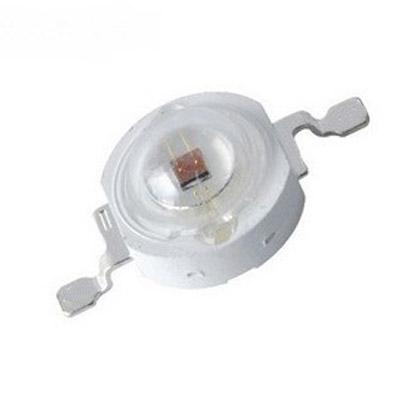
\includegraphics[width=5cm]{img/LED.png}
\caption{Svjetleća dioda visoke snage\protect\footnotemark}
\label{fig:LED}
\end{figure}
\footnotetext{Izvor: http://www.ledlightmake.com/bmz\_cache/infrared\%20850nm\%20led\%203W.jpg}\\
One su postavljene na gornji dio heksakoptera, a napajaju se iz baterije koja pokreće motore samog heksakoptera. Potrebno je koristiti što lakše dijelove kako težina ne bi previše utjecala na samo upravljanje. Modificirani heksakopter može se vidjeti na \ref{fig:modificirani dron}.
\begin{figure}[htb]
\centering
\begin{subfigure}{.48\textwidth}
  \centering
  \includegraphics[width=.9\linewidth]{img/dron_gore.JPG}
  \caption{Gornji dio - vidljive svjetleće diode}
  \label{fig:gornji}
\end{subfigure}
\begin{subfigure}{.48\textwidth}
  \centering
  \includegraphics[width=.9\linewidth]{img/dron_dole.JPG}
  \caption{Donji dio - spajanje na bateriju}
  \label{fig:donji}
\end{subfigure}
\caption{Modificirani dron - dodane infracrvene svjetleće diode}
\label{fig:modificirani dron}
\end{figure}


\subsection{Sustav kamera}\label{sec:kamera}
Za točno određivanje položaja heksakoptera u prostoru potreban je sustav kamera. Postoje mnoge skupe kamere za praćenje letjelica, poput poznatog OptiTrack sustava, no u ovom eksperimentu potrebno je koristiti neku jeftiniju inačicu. Tako se može koristiti Wii Remote (prikazan slikom \ref{fig:Wii Remote}) u kojeg je ugrađena infracrvena kamera ili Pixy (prikazana slikom \ref{fig:Pixy kamera}) kamera s lećom koja uočava infracrveno svijetlo. 
\begin{figure}[htb]
\centering
\begin{minipage}{.4\textwidth}
  \centering
  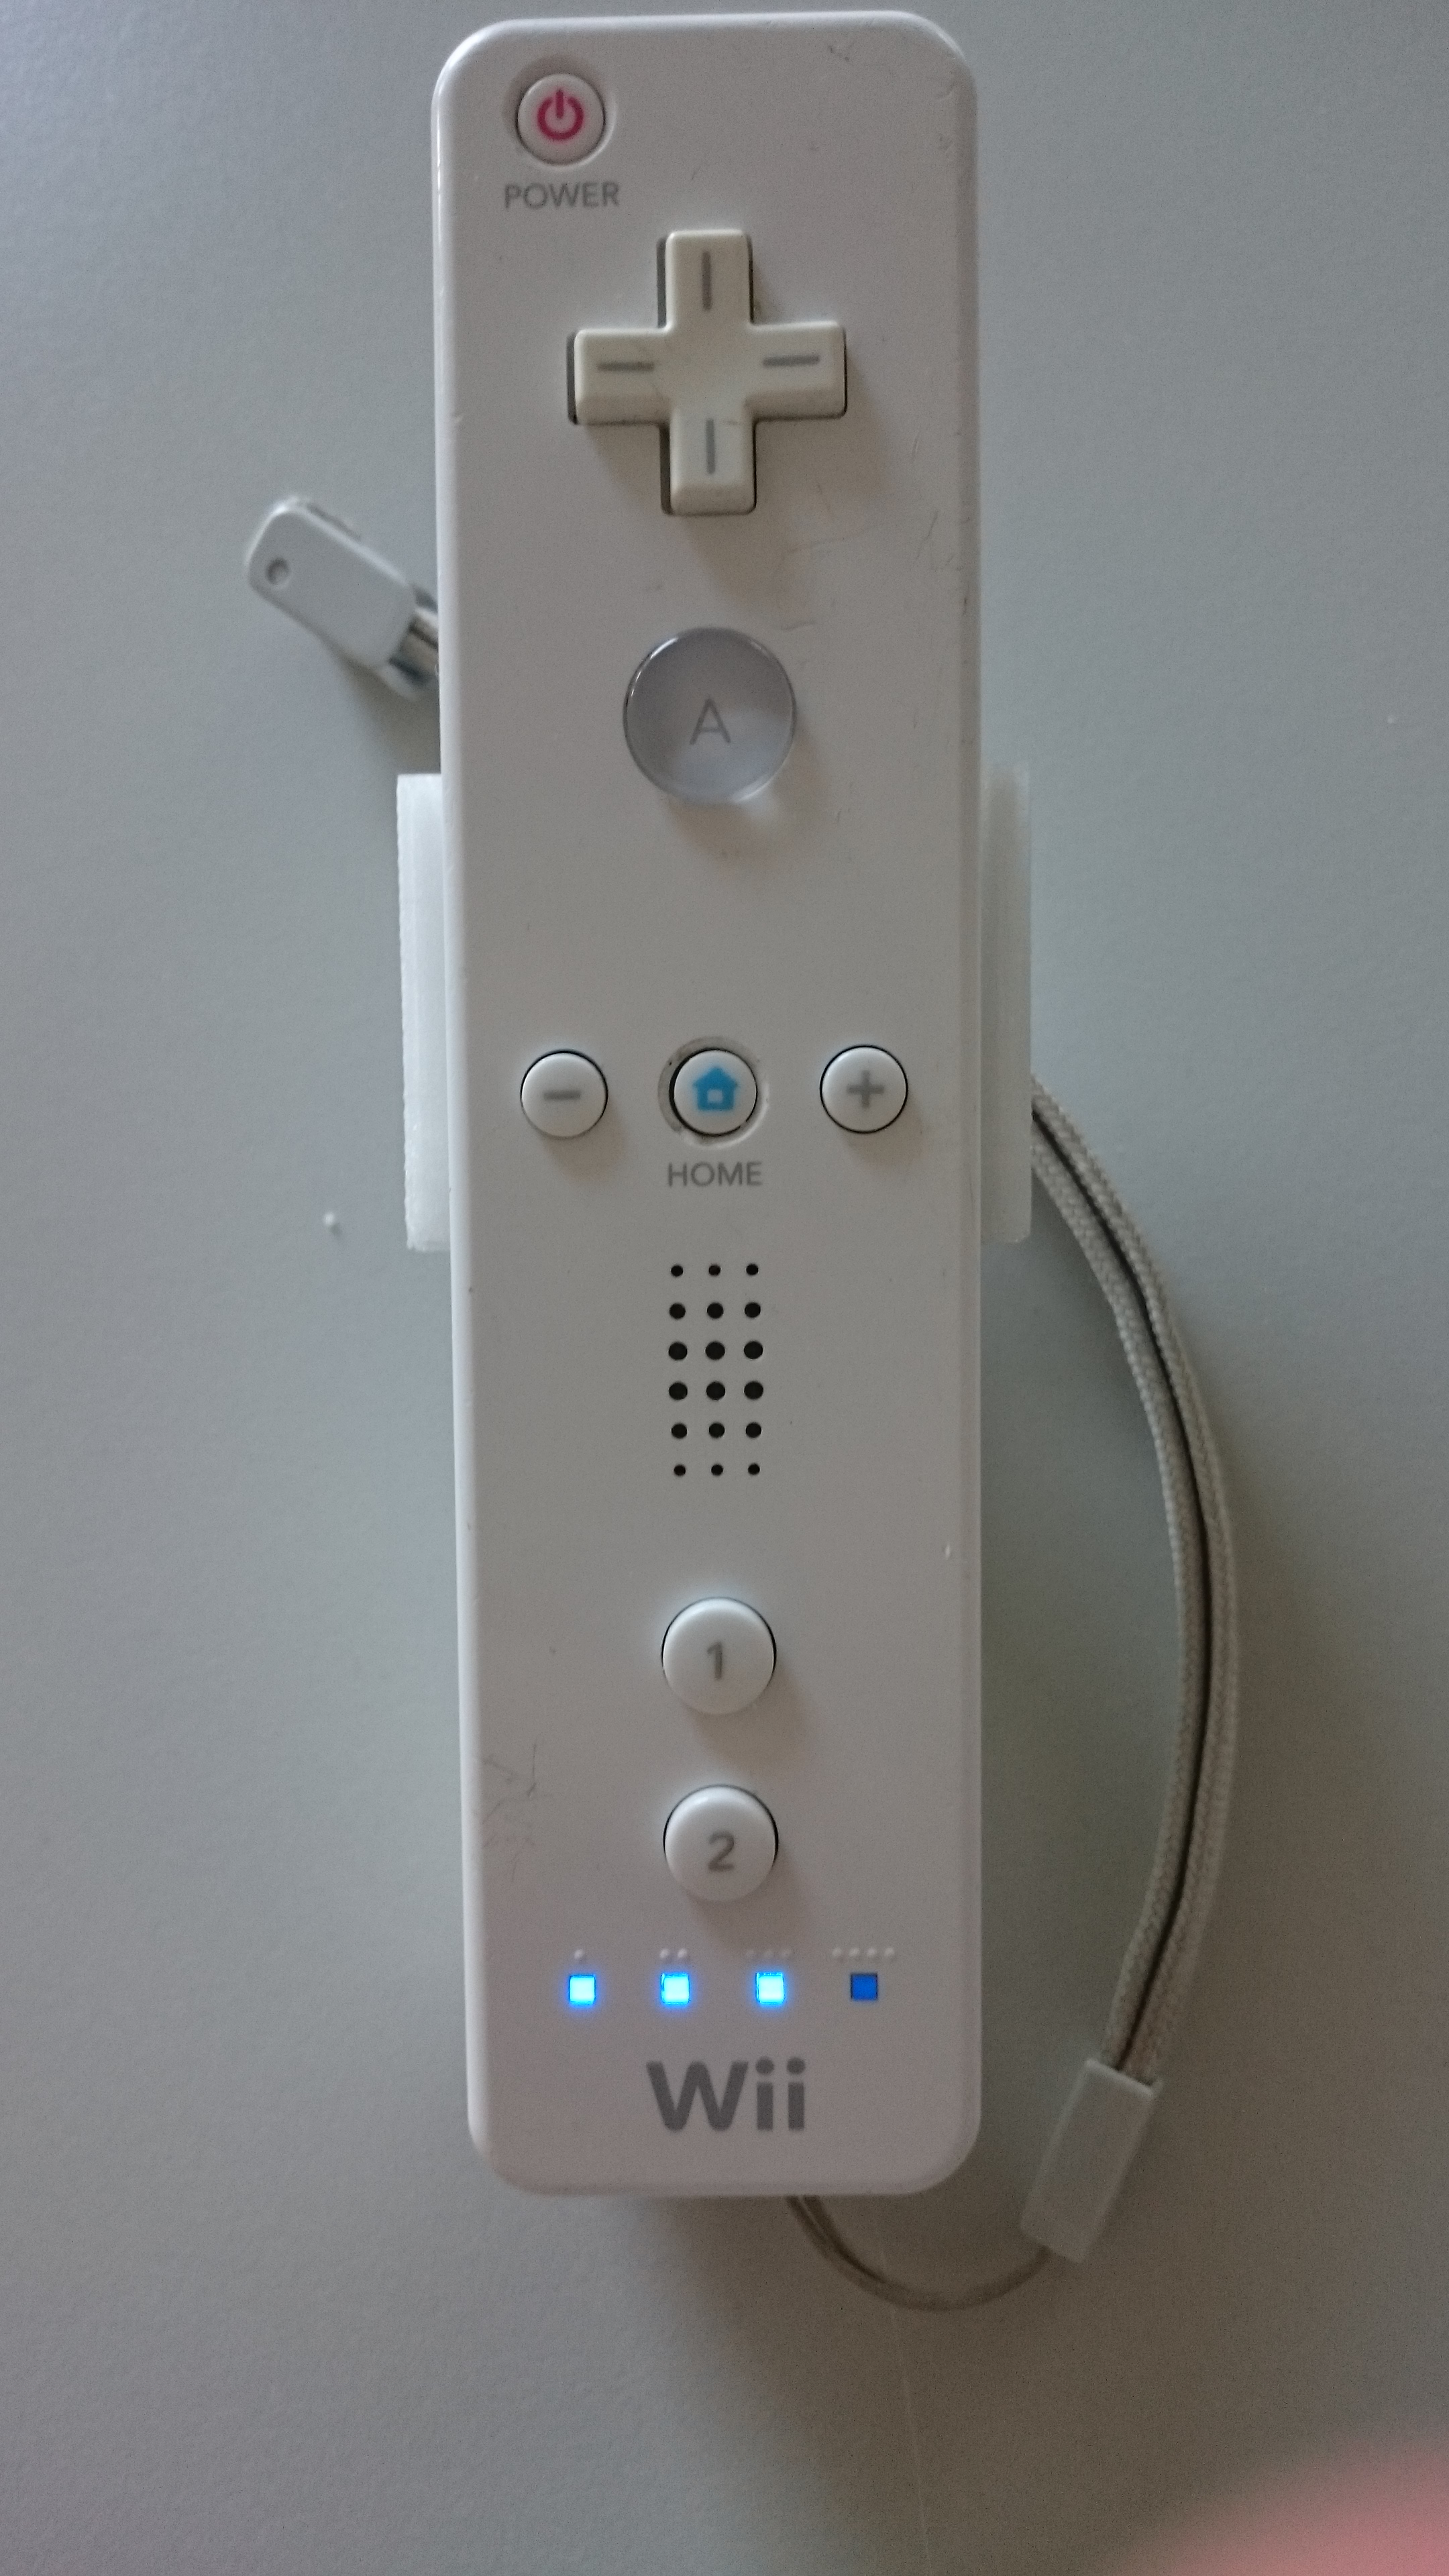
\includegraphics[width=.5\linewidth]{img/wiimote.JPG}
  \captionof{figure}{Wii Remote}
  \label{fig:Wii Remote}
\end{minipage}%
\begin{minipage}{.5\textwidth}
  \centering
  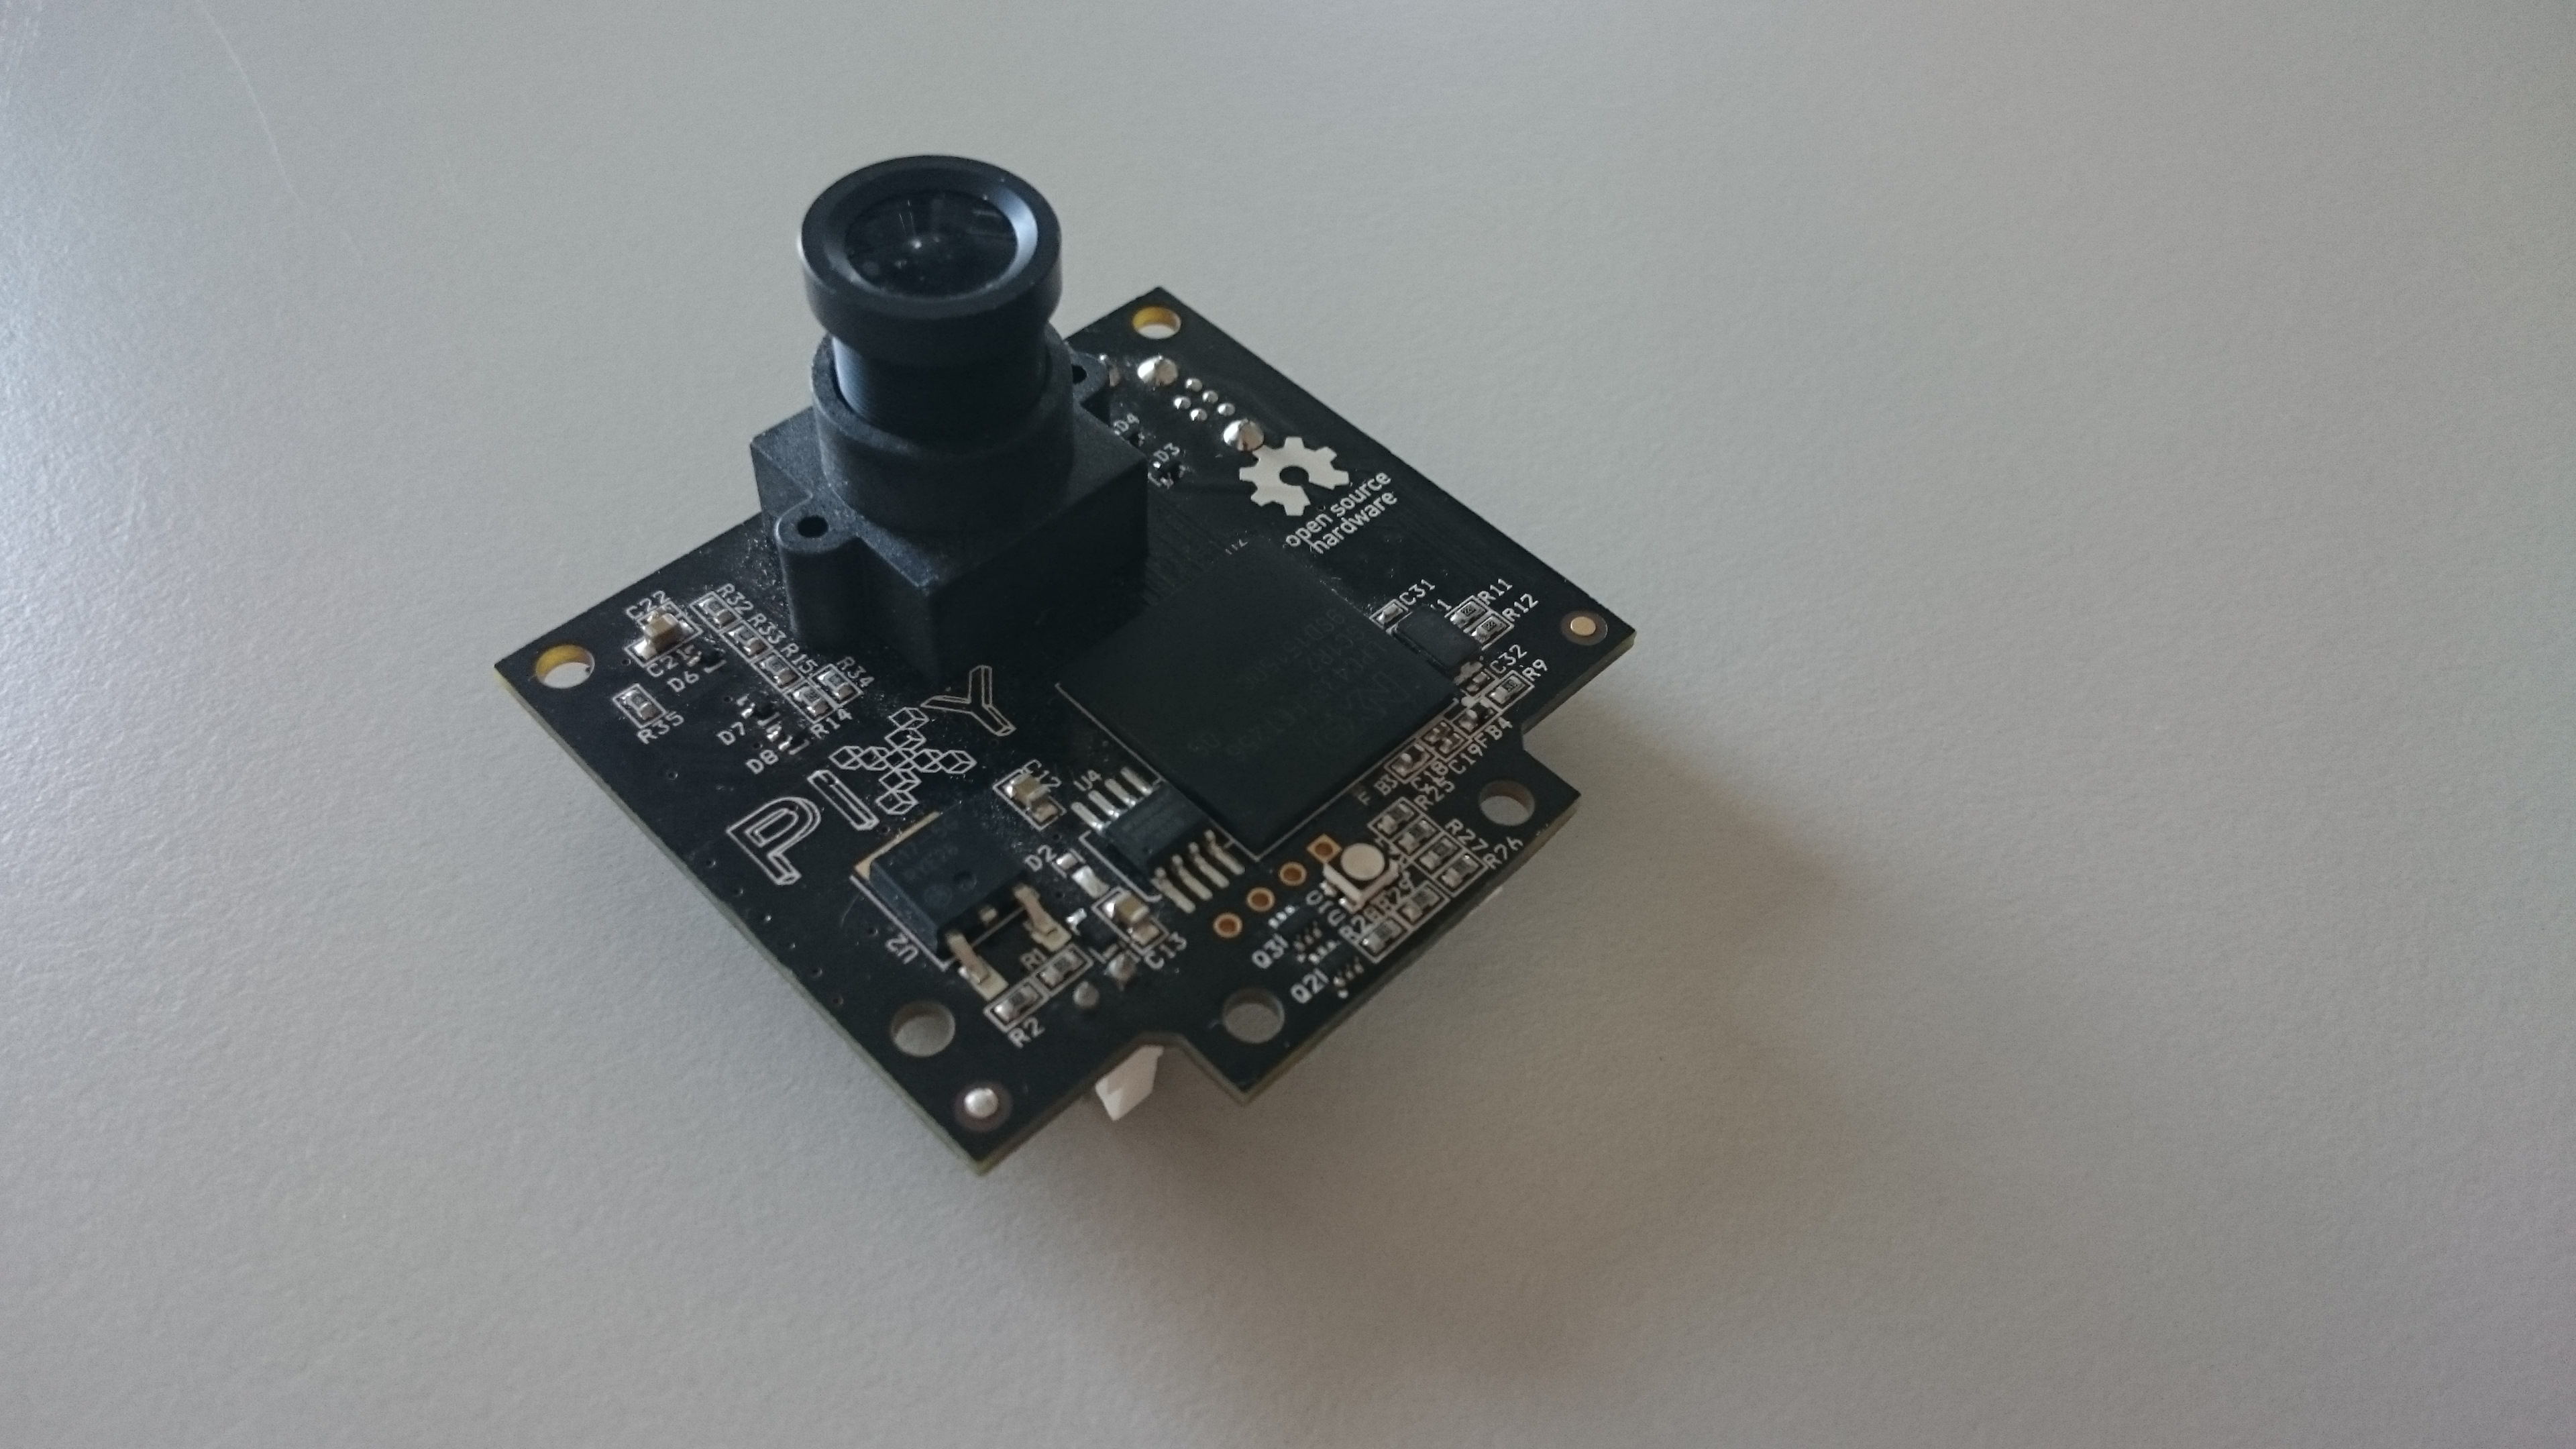
\includegraphics[width=.9\linewidth]{img/pixy.JPG}
  \captionof{figure}{Pixy kamera}
  \label{fig:Pixy kamera}
\end{minipage}
\end{figure}
Sustav kamera je točno određen (zadani položaj i orijentacija kamera) tako da preko fiksnih matrica transformacija daje informaciju o poziciji i orijentaciji samog drona. Ova dobivena informacija se dalje koristi se u računalu prilikom zadavanja upravljačke veličine za upravljanje heksakopterom (više o upravljanju u \ref{sec:algoritam}).

\subsection{Kontroler i njegova modifikacija pomoću Arduina}\label{sec:kontroler}
U ovom poglavlju prikazana je modifikacija kontrolera kako bi se omogućilo slanje upravljačkih signala iz računala preko kontrolera na dron. Kako se putem \emph{gljiva} upravlja dronom, odnosno lijevom gljivom se zadaju potisak \engl{thrust} i zakret \engl{yaw} te desnom gljivom pomak naprijed-nazad i pomak lijevo-desno, potrebno je omogućiti da se upravljačke veličine koje izlaze iz tih \emph{gljiva} zadaju preko računala. Pošto su \emph{gljive} zapravo potenciometri u vertikalnom i horizontalnom smjeru, promjenom njihovog položaja mijenja se  upravljačka veličina. Signali koje generira kontroler su analogni. Tu su 3 električna voda: GND, VCC i upravljački signal (napon na otporniku). Korištenjem multimetra identificiraju se vodovi i izmjeri se napon između upravljačkog signala i GND. U ovoj situaciji izmjereni su sljedeći naponi:
\begin{itemize}
\item 0.24 V - minimalni
\item 1.64 V - srednji
\item 3.10 V - maksimalni
\end{itemize}
Sada kada su određene veličine analognih signala potrebno je fizički prekinuti vod iz upravljačkog signala te zalemiti žice na svaki kraj tog voda, kako bi kratkospajanjem tih žica funkcionalnost kontrolera ostala ista.  To je prikazano na slikama  \ref{fig:kontrolerUnutra} i \ref{fig:kontrolerVani}.
\begin{figure}[htb]
\centering
\begin{minipage}{.6\textwidth}
  \centering
  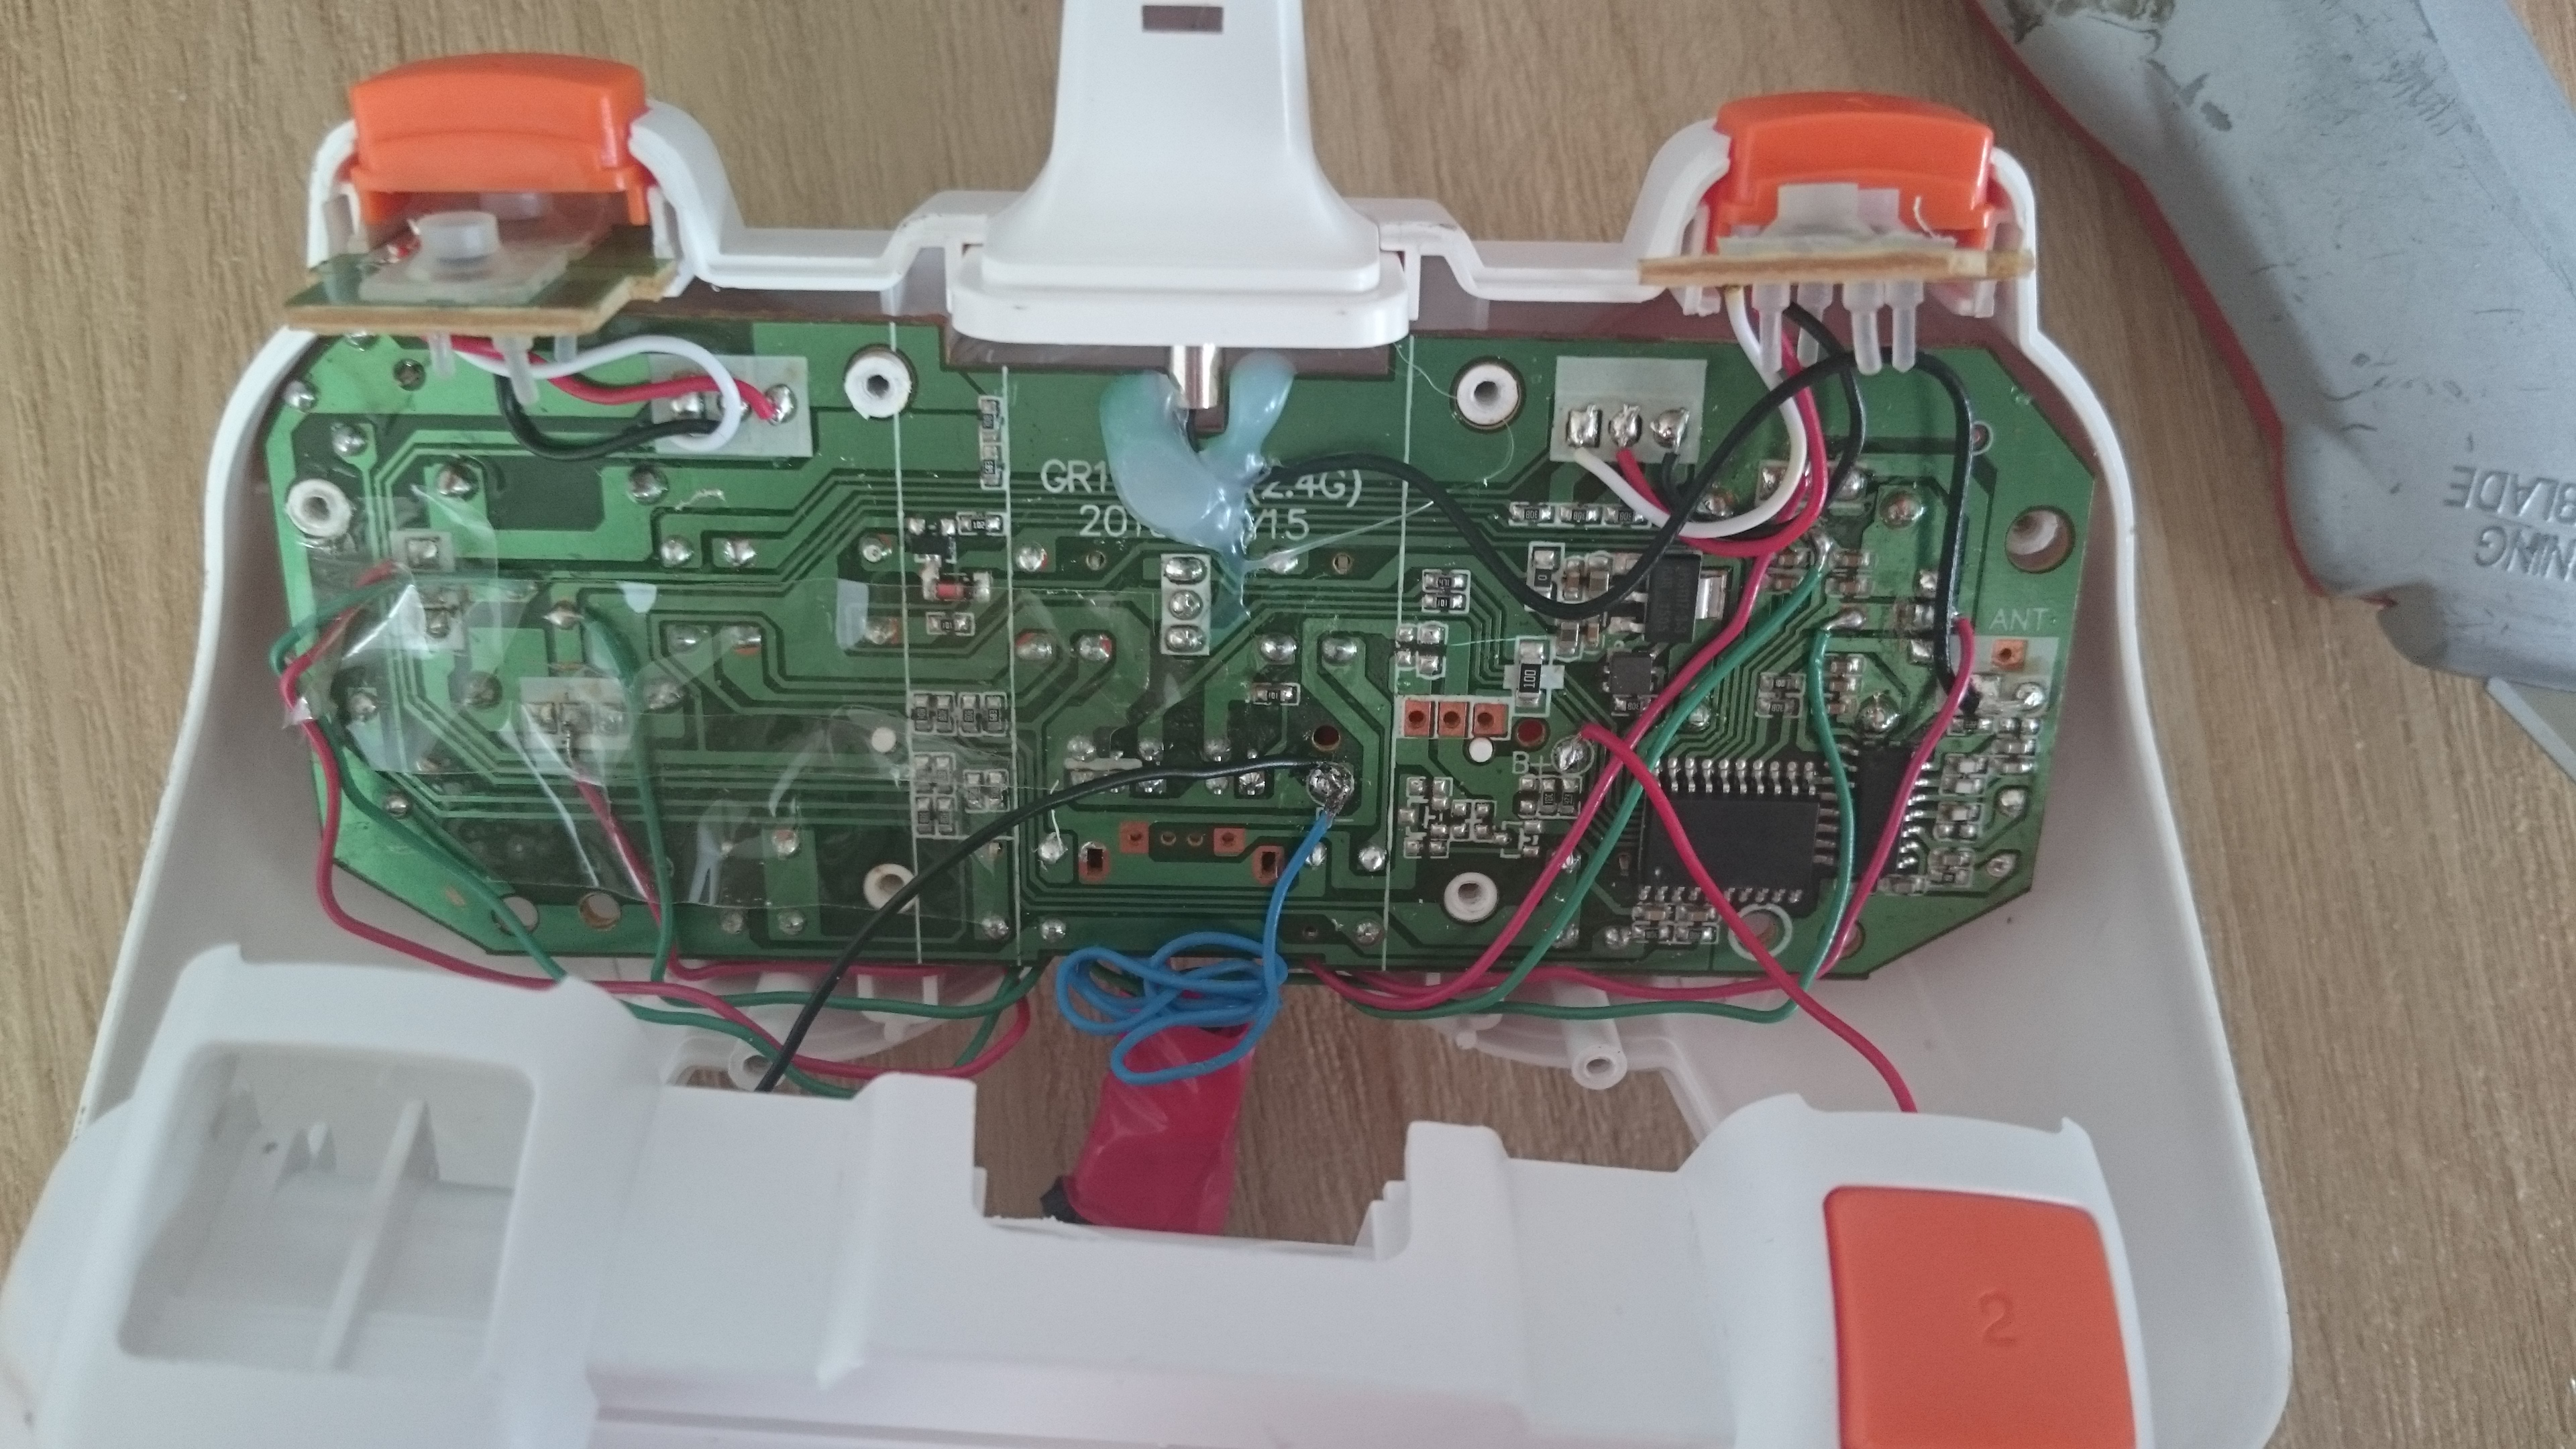
\includegraphics[width=.8\linewidth]{img/modificiranje.JPG}
  \captionof{figure}{Modificiranje kontrolera}
  \label{fig:kontrolerUnutra}
\end{minipage}%
\begin{minipage}{.4\textwidth}
  \centering
  \includegraphics[width=.5\linewidth]{img/modificirani.JPG}
  \captionof{figure}{Modificirani kontroler}
  \label{fig:kontrolerVani}
\end{minipage}
\end{figure}\\
Nakon što je sve određeno i izvedeno Arduino se spaja na kontroler. Preko Arduina se zadaju upravljački naponi, no potrebno je dodati još nekoliko elemenata. Prilikom korištenja naredbe \emph{analogWrite} Arduino generira signal koji je potreban, no na taj način se ne može upravljati dronom iako se mjerenjem tog signala ispostavlja da je točan. Zaključak je da taj signal nije dovoljno \emph{stabilan} za upravljački signal te zbog tog trebamo koristiti dodatni krug za izglađivanje. Za izglađivanje se koristi LM324AN koji sadrži 4 operacijska pojačala, jer je potrebno zadati 4 upravljačke veličine. Operacijskim pojačalima potrebno je prethodno staviti otpornik ($4.7k\Omega$ ) i kondenzator ($10 \mu F$). Dodano je i vanjsko napajanje koje iz \emph{mreže} preko ispravljača napona ispravlja napon na istosmjernih 12V nakon čega se preko stabilizatora napona stabilizira napon na 5V te se takav koristi za operacijska pojačala i Arduino. Između ulaza i GND stabilizatora stavlja se kondenzator od $10\mu F$, a između izlaza i GND stabilizatora kondenzator od $1\mu F$. Na ulaz LM324AN dovodi se upravljački signal generiran Arduinom te se takav izglačani signal dovodi na dronov kontroler. Način spajanja prikazan je na slici \ref{fig:spajanje}.
\begin{figure}[htb]
\centering

\includegraphics[width=5cm]{img/fer_logo.jpg}
\caption{Način spajanja Arduina i kontrolera\protect\footnotemark}
\label{fig:spajanje}
\end{figure}
\footnotetext{niš}
Jedna bitna stvar za napomenuti je kako svi dronovi trebaju primiti od kontrolera signal za buđenje \engl{Wake up signal}, koji je drugačiji za različite proizvođače, kako bi se s njime moglo upravljati. U ovom slučaju \emph{Wake up} signal je zadavanje maksimalne pa minimalne vrijednosti \emph{thrusta}, odnosno pomak lijeve gljive skroz prema gore pa skroz prema dolje. Također, ovaj kontroler ima opciju za fino podešavanje pa je prilikom \emph{Wake up} signala potrebno imati kratkospojene vodove kako bi se kontroler točno podesio. Ako se to ne napravi nakon simuliranog \emph{Wake up} signala, izgubi se mogućnost upravljanja drona prema naprijed i prema desno. Upravljanje preko Arduina treba biti jednako kao i fizičko upravljanje preko kontrolera, tako treba napomenuti da je prilikom slanja nove upute \engl{command} potrebno upravljački signal staviti u sredinu te ga tek zatim postaviti u drugu vrijednost (ovo vrijedi samo kod prelaska kroz srednju vrijednost). Vrlo važno je zapamtiti da se dron prvo treba prizemljiti te tek onda ugasiti motore i kontroler. Ukoliko se kontroler ugasi prilikom rada na dronu ostaju zadnje poslane upute. Time može doći do oštećenja opreme i prostora oko drona. Slikom \ref{fig:cijeli sustav} se prikazuje cijeli navedeni sustav, a poglavljem \ref{sec:algoritam} bit će opisani algoritam i softverski dio.
\begin{figure}[htb]
\centering

\includegraphics[width=5cm]{img/fer_logo.jpg}
\caption{Spajanje računala, Arduina i kontrolera\protect\footnotemark}
\label{fig:cijeli sustav}
\end{figure}
\footnotetext{niš}



\subsection{Računalo s algoritmom upravljanja}\label{sec:algoritam}
Za upravljanje se koristi robotski operativni sustav - ROS\footnote{Više informacija je dostupno na: \url{http://wiki.ros.org/}}. ROS prikuplja softverske okvire za razvoj robotskog softvera. ROS nije operacijski sustav, ali pruža usluge oblikovane za heterogene računalne skupine kao što su hardverska apstrakcija, niska razina kontrole uređaja, implementacija uobičajeno korištenih funkcija, prijenos poruka između procesa i upravljanje paketima. Obrada se odvija u čvorovima \engl{nodes} koji mogu primati, postavljati, kontrolirati,  držati i aktivirati razne informacije iz različitih senzora i aktuatora. Unatoč važnosti reaktivnosti i niske latencije u kontroli robota, tako i bespilotnih letjelica, ROS sam po sebi nije \emph{real-time} operacijski sustav, iako je moguće integrirati ROS s \emph{real-time} kodom. U ovom projektu korišteni je \emph{ROS Kinetic Kame}\footnote{Više o instalaciji na: \url{http://wiki.ros.org/kinetic/Installation/Ubuntu}} koji se može instalirati na \emph{Ubuntu  (16.04 LTS)} distribuciji \emph{Linuxa}. Nakon instalacije potrebnih paketa povezuju se čvorovi (prikazani slikom \ref{fig:cvoroviROS}) s algoritmom upravljanja te se uspostavlja komunikacija između Arduina i ROS-a.
\begin{figure}[htb]
\centering

\includegraphics[width=5cm]{img/fer_logo.jpg}
\caption{Shema ROS čvorova}
\label{fig:cvoroviROS}
\end{figure}

\subsubsection{Implementacija PID regulatora}
Komponente i sam PID regulator su objašnjeni u poglavlju \ref{PIDreg}. U dodatku je kod koji prikazuje implementaciju diskretnog PID regulatora Python skriptom.
%\appendix
%\chapter{Implementacija PID regulatora}
%\lstinputlisting[language=Python]{code/pid.py}

\subsubsection{Komunikacija između Arduina i ROS-a}
Arduino se koristi za generiranje PWM signala koji se šalje na kontroler. U ovom poglavlju bit će opisan Arduino IDE program. No prvi korak je instalacija Arduino IDE te \emph{rosserial arduino} \footnote{Upute za instalaciju su dostupne na: \url{http://wiki.ros.org/rosserial_arduino/Tutorials/Arduino IDE Setup}} paketa za povezivanje ROS direktno s Arduino IDE. \emph{Rosserial} sadrži ROS komunikacijski protokol koji funkcionira preko Arduinovog serijskog porta - UART. Ovaj paket omogućuje Arduinu da bude ponopravni ROS čvor koji može izravno objavljivati i pretplatiti se na ROS informacije. Nakon što se program spusti na Arduino u terminalu se pokrene serijska komunikacija naredbom:
\begin{lstlisting}
rosrun rosserial_python serial_node.py
\end{lstlisting}
U Arduino programu se prvo definira potrebni paketi.
\lstinputlisting[language=C, firstline=1, lastline=2]{code/pid_listening.c}
Definiraju se varijable, odnosno frekvencija, inicijalne upravljačke veličine za generiranje PWM signala koji se šalje preko filtra i operacijskog pojačala na kontroler te korišteni pinovi. Arduino na svojim izlazima može dati maksimalno 5V što se postiže postavljanjem vrijednosti PWM signala na 255. Tako npr.~napon iznosa 3.10 V se postiže postavljenjem vrijednosti PWM signala na 179.
\lstinputlisting[language=C, firstline=4, lastline=17]{code/pid_listening.c}
Potrebno je definirati pretplatu \engl{subscriber} na čvor \engl{node} koji postavlja vrijednosti za generiranje PWM signal. \emph{Subscriber} ima pozivajući funkciju koja kod promjene u čvoru uzima vrijednosti i sprema ih u varijable.
\lstinputlisting[language=C, firstline=22, lastline=32]{code/pid_listening.c}
U \emph{setup} funkciji, koja se izvršava samo kod pokretanja, definiraju se svi pinovi kao izlazni \engl{output}. Potrebno je namjestiti PWM frekvenciju, odnosno povećati ju kako bi signal bio stabilniji. Za ispravljanje PWM signala na pinovma 9 i 10 koristi se brojač 1, dok se za pinove 11 i 3 koristi brojačem 2. PWM frekvencija iznosi 3921.16 Hz. Također je potrebno jednom inicijalizirati ROS čvor za obradu, 
\lstinputlisting[language=C, firstline=33, lastline=44]{code/pid_listening.c}
Glavna petlja zadanom frekvencijom postavlja nove vrijednosti PWM signala.
\lstinputlisting[language=C, firstline=45, lastline=58]{code/pid_listening.c}

\subsubsection{Algoritam upravljanja}
Sam algoritam upravljanja opisan je Python skriptom. Implementirana je samo vanjska petlja, odnosno upravljanje po poziciji i orijentaciji. Unutarnja petlja je implementirana već u samom dronu izvršavajući komande koje šalje kontroler. Način na koji je ona implementirana je nepoznanica pošto ne postoji neki opširni\emph{manual} za korišteni dron. Nadalje, u ovom programu se povezuju svi čvorovi sa sheme \ref{fig:cvoroviROS}. Program sadrži 3 pretplatnika, te 2 objavljivača \engl{publisher}:
\begin{itemize}
\item Subscriber "drone/pose\_ref" --- referentna pozicija i orijentacija
\item Subscriber "drone\_position" --- izmjerena pozicija i orijentacija
\item Subscriber "keyboard" --- kontrola preko tipkovnice
\item Publisher "control/drone\_input" --- upravljačka veličina koja se šalje na Arduino
\item Publisher "pose\_error" --- pogreška pozicioniranja
\end{itemize}
U prethodnom poglavlju opisan je pretplatnik na čvor "control/drone\_input" (Arduino program), a u nastavku je programskim kodom opisani objavljivač na taj isti čvor (algoritam upravljanja). 
\lstinputlisting[language=Python, linerange={57-59,189-190}]{code/pid_controller.py}
Ovime je pokazano kako lako, u ROS-u preko čvorova, mogu dva zasebna programa komunicirati jedan između drugog.
Za upravljanje vanjskom petljom potrebna su 4 PID regulatora za upravljanje po X, Y, Z poziciji te orijentaciji \emph{yaw}. No prije parametriziranja regulatora potrebno je izmjeriti potisak na kojem dron lebdi. Za tu priliku se preko tipkovnice zadaje ručno upravljačka veličina koja će osigurati lebdenje drona. Osim za zadavanje upravljačkog signala, tipkovnica se koristi i kod pripreme hardvera, tj.~pritiskom na tipku daje se signal da se algoritam može pokrenuti. Uz to se preko tipkovnice zbog sigurnosti, odnosno mogućeg neočekivanog rada, mogu isključiti svi motori. Ova funkcionalnost je potrebna jer se na drugi način ne mogu isključiti motori. Razlog tome je što dron izvršava onu naredbu koju je zadnju prihvatio od kontrolera, pa se onda može samo fizički zaustaviti. 
\lstinputlisting[language=Python, linerange={137-139}]{code/pid_controller.py}
Za čitanje s tipkovnice koristi se paket \emph{pynput} koji je potrebno prethodno instalirati.
Koristi se diskretizirani PID regulator  čija izvedba je prikazana u dodatku, a potrebno ga je ubaciti \engl{import} u Python skriptu.  Prilikom pokretanja jednom se inicijaliziraju PID kontroleri. 
\lstinputlisting[language=Python, linerange={30-33}]{code/pid_controller.py}
Ovdje se parametri (koeficijenti) određuju eksperimentalno. 
Petlja, odnosno algoritam koji se stalno vrti je prikazan sljedećim isječkom koda. Na vrijednost potiska ne utječe orijentacija pa ga je najlakše odrediti. U ovisnosti o orijentaciji potrebno je dobro namjestiti, preko geometrije, veličine za kontrolu u odnosu na X i Y os.   
\lstinputlisting[language=Python, linerange={123-170,189-190}]{code/pid_controller.py}
Također dodani je predfilter za filtriranje reference i mjernih podataka.
\begin{lstlisting}
def prefilter(x_k, x_k_1, a):
	""" First order filter.
	:param x_k: Current value
	:param x_k_1: Previous value
	:param a: Filter constant	"""
	
	return (1 - a) * x_k_1 + a * x_k \end{lstlisting}


\subsubsection{Redoslijed pokretanja}
\begin{enumerate}
	\item Pokreće se terminal te zatim ROS naredbom
	\begin{lstlisting}
	roscore	\end{lstlisting}
	\item Pokreće se serijska komunikacija između računala i Arduina
	\begin{lstlisting}
	rosrun rosserial_python serial_node.py	\end{lstlisting}
	\item Spajaju se WiiMote-vi koji služe kao indikatori položaja (nakon naredbe potrebno je stisnuti tipke 1 i 2 na WiiMotu). Paket je modificiran tako da se prilikom spajanja proslijeđuje ID zbog razlikovanja čvorova.
	\begin{lstlisting}
	rosrun wiimote wiimote_node2.py _id:=1
	rosrun wiimote wiimote_node2.py _id:=2	\end{lstlisting}
	\item Pokretanje neuronske mreže koja iz podataka iz WiiMote-ova izračunava točan poziciju i orijentaciju.
	\begin{lstlisting}
	rosrun diplomski wii_neural.py \end{lstlisting}
	\item Kontroler se postavlja tako da šalje vrijednosti koje su na kontroleru (zbog početnog kalibriranja prilikom \emph{wake up} signala). Dron se uključuje te se izvodi \emph{wake up} signal. Nakon povezivanja kontrolera i drona tako da kontroler prihvaća vrijednosti od računala pokreće se algoritam upravljanja i čitač s tipkovnice.
	\begin{lstlisting}
	rosrun diplomski pid_controller.py
	rosrun diplomski keyboard.py \end{lstlisting}
\end{enumerate}


\subsection{Rezultati}
 


\chapter{Zaključak}
Upravljanje dronom izvršeno je na relativno jeftinoj opremi. Dron je malih dimenzija i male snage što uvelike utječe prilikom dodavanja dodatnog tereta na njega (dodavanjem LED indikatora promijenio se centar mase pa tako i dinamika samog drona). Detekcija pozicije dobiva se preko jeftinog WiiMota, u odnosu na profesionalnije kamere koje su puno skuplje, što utječe na točnost mjerenja i na veličinu radnog prostora. Radni prostor je relativno mali. Iako je zadovoljio potrebe eksperimenta za neke ozbiljnije testove i trajektorije potrebni je ipak nešto veći radni prostor. Problem nešto lošijeg indikatora mogao bi se riješiti estimacijom pozicije drona, no u ovom slučaju teško je odrediti točan matematički model, zbog promjena centra mase, momenata inercije, koji bi Kalmanofiltar koristio za estimaciju stavljajući veću težinu na dobiveni matematički model. Prethodno navedene promjene trebalo bi kompenzirati u unutarnjoj upravljačkoj petlji koja je riješena već u samom kontroleru i dronu te se stoga ne može mijenjati, tj.~korisnik nema pristupa. Kako se ne bi previše promijenila masa drona dodavanjem nove baterije, koja je potrebna za napajanje LED indikatora, korištena je postojeća koja napaja i motore. Kako su LED indikatori velike snage, baterija je dodatno opterećena što ima nekog utjecaja na snagu motora. Iz eksperimenata se može uočiti da se dron ne ponaša jednako prilikom različitih razina napunjenosti baterije. Samim time što je činjenica da se dronom upravlja preko kontrolera, ne može se sa sigurnošću potvrditi kako se promjena upravljačke veličine u kontroleru izvrši na dronu, tj.~da li je linearnom promjenom upravljačke veličine i odziv linearan. Rješenje ovog problema, što je ujedno i nastavak budućeg razvoja, jest izrada većeg drona (što znači i težeg koji će manje promijeniti centar mase dodavanjem indikatora), sa snažnijim motorima koji neće osjetiti promjenu mase te vlastitim sklopovljem koje će izvršavati algoritam upravljanja unutarnje petlje (postoje \emph{open-source} algoritmi koji se mogu lako modificirati). Prilagođavanjem unutarnje i vanjske petlje upravljanja dolazi se do srži problema, te su mogući i napredniji načini upravljanja.

\vfill
\hspace*{0pt}\hfill Potpis:  $\_\_\_\_\_\_\_\_\_\_\_\_\_\_\_\_\_\_\_\_\_$\\
\hspace*{5pt}\hfill Luka Galović

\bibliographystyle{fer}
\bibliography{literatura}

\appendix
\chapter{Python implementacija PID regulatora}
\lstinputlisting[language=Python]{code/pid.py}


\begin{sazetak}
Bespilotne letjelice imaju sve veću upotrebu i važnost u svakodnevnom životu. Kroz povijest se mijenjala njihova upotreba pa postoji nekoliko vrsta. Sve većom upotrebom u poljoprivredi, geodeziji te za zabavu javila se potreba za zakonskom regulativom. Najveći izazov kod bespilotnih letjelica je njihovo upravljanje i točno pozicioniranje. Za rješavanje tog problema potrebno je dobro odrediti matematički model za sintezu sustava upravljanja. Model heksakoptera je izveden korištenjem Newtonovih zakona. Korištenjem kvaterniona, u odnosu na Eulerove kutove, smanjuje se nestabilnost te ubrzava numerički izračun. Projektirani regulator za slijeđenje željene trajektorije ima raspoložive informacije o trenutnoj poziciji i orijentaciji letjelice. Glavno svojstvo letjelica je njihova nestabilnost. Kako bi se upravljalo preko računala, modificirani je kontroler heksakoptera tako da Arduino, uz dodatne elemente za filtriranje signala, generira upravljački signal. Algoritam upravljanja implementiran je u robotski operativnom sustavu - ROSu. Na kraju su prikazani rezultati algoritma. 

\kljucnerijeci{Bespilotne letjelice, upravljanje, matematički model, heksakopter, kvaternioni, Eulerovi kutovi, trajektorija, Arduino, ROS.}
\end{sazetak}
\newpage
% TODO: Navedite naslov na engleskom jeziku.
\engtitle{Design of a Path Tracking Controller for Unmanned Aerial Vehicle in Global Vision System}
\begin{abstract}
The use and importance of unmanned aerial vehicles are increasing in everyday life. Throughout history, their use has been changed and there are several types. Legal regulations had to be published because of their increasing use in agriculture, geodesy and for entertainment. The biggest challenge for unmanned aerial vehicles is control and accurate positioning.
To solve this problem, it is necessary to define a mathematical model for the synthesis of the control system. The model of flying hexacopter is derived using classical Newton laws. By using quaternions, relative to the Euler angles, instability decreases and the numerical calculations accelerate. The designed controller for the trajectory tracking has available information on the current position and orientation of the aircraft. The main property of such devices is their instability. In order to control the hexacopter from the computer, the hexachopter controller is modified so that an Arduino, with some additional elements for filtering signals, can generate a control signal. Algorithm for control is implemented in the robotic operating system - ROS. Results of the control algorithm are presented in the end of the paper.

\keywords{Unmanned Aerial Vehicle, control, mathematical model, hexacopter, quaternions, Euler angles, trajectory, Arduino, ROS.}
\end{abstract}\\


\end{document}
